% ------------------------------------------------------------------------------
% Investigation
% ------------------------------------------------------------------------------

\chapter{Investigation}\label{chap:investigation}

	%Após as discussões sobre a teoria do problema e as metodologias mais conhecidas na literatura, este capítulo se propõem a ressaltar as oportunidades de contribuição e o projeto de pesquisa deste doutorado. Primeiramente, além de destacar quais tópicos devem ser mais explorados nas próximas publicações na literatura, é feita uma discussão crítica de alguns pontos da literatura e as oportunidades que essas lacunas representam. A partir dessas oportunidades, a pesquisa é delimitada contendo três frentes de investigação. Em cada uma delas é reforçada as contribuições esperadas. Por fim, a conclusão retoma os principais pontos do capítulo, destacando as técnicas implementadas.
	After discussions about the problem theory and the most well-known methodologies in the literature, this chapter highlights the opportunities for contribution and the research project of this doctorate. First, in Section \ref{chap:investigation:criticism}, besides underscoring which topics should be further explored in future publications in the literature, there is a critical discussion of some points in the literature and the opportunities these gaps represent. From these opportunities, the research is delimited in Section \ref{chap:investigation:proposal}, containing three research fronts. In each of them, the expected contributions are reinforced. Finally, the conclusion returns to the main points of the chapter, highlighting the techniques implemented (Section \ref{chap:investigation:conclusion}).

	\section{Literature Criticism and Opportunities}\label{chap:investigation:criticism}
	
		%O alvo do desenvolvimento de metodologias para o imageamento em microondas é avançar na qualidade das reconstruções e nos custos das metodologias, i.e., recuperar imagens em alta resolução e se basear em operações rápidas que possiblitem o imageamento tempo real. É claro que a má-posição do problema sempre vai ser um obstáculo que imporá limites às aplicações. No entanto, isto não tem impedido o progresso das técnicas. Por isso, melhorias nos métodos determinísticos e estocásticos já existentes são possíveis, assim como metodologias totalmente novas. Não somente metodologias, mas também estratégias que potencializarão os métodos já existentes. Do ponto de vista do autor desta dissertação, três estratégias mencionadas nos capítulos anteriores serão muito exploradas nos próximas metodologias:
		The aim of developing methodologies for microwave imaging is to advance the quality of the reconstructions and the costs of the methodologies, i.e., recovering high-resolution images and relying on rapid operations that enable real-time imaging. The ill-posedness condition will always be an obstacle that will impose limits on the applications. However, this has not hindered the progress of the techniques. Therefore, improvements in existing deterministic and stochastic methods are possible, as well as new methodologies. Not only methodologies but also strategies that will enhance existing methods. There are expectations on three strategies mentioned in the previous chapters that will be explored in the future methodologies:
		
		\begin{itemize}
			%\item Deep-Learning: foi notória a contribuição desta técnica para o problema. Sua inserção possibilitou avanços especialmente na capacidade de reconstruir bem os contornos dos objetos além de reduzir tempo de execução tomando como base a rede já treinada.
			\item Deep-Learning: the contribution of this technique to the problem was notorious. Its insertion enabled advances, especially for better reconstruction of objects contour and reducing execution time based on the already-trained network.
			%\item Contraction Integral Equation: a definição do problema em termos da integral \eqref{eq:2:eisp:9} trouxe avanço significativo na reconstrução de espalhadores fortes.
			\item Contraction Integral Equation: the definition of the problem in terms of the integral \eqref{eq:2:eisp:9} has brought a significant advance in reconstructing strong scatterers.
			%\item Iterative Multi-Scaling Approach: embora este autor não acredite que novas mudanças serão propostas nesta técnica (visto que ela já foi repetida de maneira igual em vários trabalhos citados no capítulo anterior), é necessário registrar a relevância que a eliminação inteligente de áreas de fundo tem para a diminuição do problema. Isso tem consequências importante tanto na rapidez das metodologias quanto na possibilidade de reconstruir imagens com mais detalhes.
			\item Iterative Multi-Scaling Approach: the strategy for background area elimination is a relevant contribution. It has significant consequences both in the speed of the methodologies and the possibility of reconstructing images in more detail. Although the authors have never proposed changes, they have explored its application in other methodologies rather than EAs.
		\end{itemize}
	
		%Essas três estratégias refletem três ideias gerais que são promissoras: aprendizagem, modificação da equação integral e eliminação de regiões. A expectativa é que reaplicações ou modificações nessas estratégias sejam consideradas nas próximas publicações. Conforme já mencionado nos capítulos anteriores, oportunidades possíveis nessa área são: o uso de de GANs, definição adaptativa de $\beta$ em \eqref{eq:2:eisp:9} e formas mais eficientes de filtragem e identificação de objetos na imagem.
		These three strategies reflect three general ideas that are promising: learning, modifying the integral equation, and eliminating regions. The expectation is that reapplications or modifications to these strategies will be considered in the next studies. As already mentioned in previous chapters, possible opportunities in this area are using GANs, an adaptive definition of $\beta$ in \eqref{eq:2:eisp:9}, and more efficient ways of filtering and identifying objects in the image.
		
		%Especificamente sobre EAs, depois de \citep{salucci2017multifrequency}, não houveram avanços significativos na otimização simultâneamente do contraste e campo. Na verdade, os trabalhos a partir de 2018 simplesmente exploraram outros mecanismos aplicados em situações de espalhadores fracos ou com a ajuda de resolvedores diretos dentro do algoritmo \citep{etminan2018electromagnetic,yang2021fft,yang2021hybrid}. O grande desafio é o grande número de variáveis que uma abordagem simultâneamente implica, o qual talvez seja o motivo pelo qual essas técnicas não têm recebido tanta atenção na literatura ultimamente. Embora o IMSA seja um importante recurso para esse tipo de situação, as técnicas de Otimização Global em Larga Escala (LSGO) podem ser uma alternativa a ser explorada. Uma das mais populares é o Algoritmo Cooperativo Co-Evolucionário  que se baseia na decomposição do problema e na evolução cooperativa entre as partes do problema \citep{ma2019survey}.
		Specifically about EAs, after \citep{salucci2017multifrequency}, there were no significant advances in the simultaneous optimization of contrast and field. In fact, the works from 2018 onwards have only explored other mechanisms applied in situations of weak scatterers or with the help of direct solvers within the algorithm \citep{etminan2018electromagnetic,yang2021fft,yang2021hybrid}. The big challenge is the large number of variables that a simultaneous approach implies, which is perhaps why these techniques have not received so much attention in the literature lately. Although IMSA is an essential resource for this kind of situation, Large-scale Global Optimization (LSGO) techniques can be an alternative to be explored. One of the most popular is the Co-Evolutionary Cooperative Algorithm, which is based on the decomposition of the problem and the cooperative evolution between the parts of the problem \citep{ma2019survey}.
		
		%Além do grande número de variáveis, outro desafio é desenvolver operadores que aproveitem dos conceitos físicos do problema. As far this author knows, nenhum trabalho de otimização simultâneamente considerou as relações físicas entre contraste e campo em seus operadores de exploração de soluções. Desta forma, quando um novo indivíduo é gerado, a pertubação em um elemento não leva em consideração a informação dos vizinhos, seja nas variáveis de contraste como nas de campo. Além disso, não foram propostas ainda técnicas que façam ligações entre as variáveis de contraste e campo quando uma destas sofre pertubação. Em outras palavras, uma pertubação que é feita na imagem de contraste do indivíduo não é levada em consideração nas pertubações da informação de campo. Tampouco existe ligação as pertubações feitas nos diferentes ângulos de incidência que compõem as variáveis de campo. O desenvolvimento de operadores de cruzamento ou de mutação que promovam variações mais inteligentes aproveitando das relações físicas entre as variáveis seria um grande avanço na aplicação de EAs para EISP.
		In addition to many variables, another challenge is to develop operators who take advantage of physical concepts. As far as this author knows, no simultaneous optimization approach has considered the physical relationships between contrast and field in their exploration operators. In other words, a perturbation made in the individual's contrast image is not taken into account in the perturbations of the field information. Nor is there any connection with the perturbations made at the different incidence angles of the field variables. The development of crossover or mutation operators that promote more intelligent modifications taking advantage of the physical relationships between the variables would significantly advance in the application of EAs for EISP.
		
		%Outro aspecto que chama a atenção na literatura é o design dos experimentos e a avaliação da qualidade dos algoritmos. É necessário destacar que um aspecto extremamente relevante para a experimentação é a utilização de modelos de espalhadores mais realísticos ou dados obtidos de medições reais. Isto tem ficado popular na literatura através laboratórios que disponibilização os dados. Dois exemplos muito comuns são o \textit{UWCEM Numerical Breast Phantom Repository} \citep{burfeindt2012mri} e as medições realizadas pelo \textit{Institut Fresnel} \citep{geffrin2005free}. 
		Another aspect that draws attention in the literature is experiment design and quality evaluation of algorithms. It is necessary to highlight that a highly relevant aspect of experimentation is using more realistic scatterer models or data obtained from real measurements. This has become popular in the literature through laboratories that make the data available. Two widespread examples are the \textit{UWCEM Numerical Breast Phantom Repository} \citep{burfeindt2012mri}  and the measurements made by the \textit{Institut Fresnel} \citep{geffrin2005free}.
		
		In addition, \cite{kurrant2021evaluating} have recently proposed a methodology to evaluate the performance of the algorithms applied to breast cancer detection. Given a reference image and the recovered one, the authors proposed to segment the tissues in the images by an unsupervised machine learning approach. After decomposing the images and mapping the tissues, five metrics were proposed to evaluate shape fidelity, malignant tissue reconstruction in tumor regions, among others. Therefore, the novelty is a technique to measure the quality of breast reconstruction with suitable tools. Their methodology is also available as a MATLAB toolbox \citep{kurrant2021mwsegeval}.
		
		%No entanto, os autores das publicações tradicionalmente escolhem instâncias com características particulares com o objetivo de demonstrar a capacidade de reconstrução do método proposto na correspondente situação. A partir disso, a performance é medida através de algum indicador de qualidade e o resultado é comparado a outros algoritmos e formulações \citep{zhong2020multiresolution,zhang2020wavelet,zhou2021improved}. Embora essa abordagem seja interessante para ilustrar a capacidade do algoritmo, ela tem pouco rigor metodológico para oferecer respostas robustas à perguntas como: (i) qual impacto da escolha da instância no valor do quantificador da performance? (ii) Como o indicador varia se a geometria do objeto mudar? (iii) Como a diferença na performance observada entre os dois métodos varia se as geometrias variarem? (iv) Qual a performance média ou pior caso do método para uma dada configuração? (v) Etc.
		However, in many publications addressing general application, traditional instances have been chosen with particular characteristics to demonstrate the reconstruction ability of the proposed method in the corresponding situation. Performance is measured through some quality indicator, and the result is compared to other algorithms and formulations \citep{zhong2020multiresolution,zhang2020wavelet,zhou2021improved}. Although this approach is interesting to illustrate the algorithm's capacity, it has little methodological rigor to offer robust answers to questions such as: (i) what is the impact of the choice of the instance on the performance quantifier's value? (ii) How does the indicator vary if the object's geometry changes? (iii) How does the difference in performance observed between the two methods vary if the geometries vary? (iv) What is the average or worst-case performance of the method for a given configuration? Among others.
		
		%Mesmo que essas perguntas possam fugir do escopo de propostas baseadas em um estudos de caso (e.g., experimentos reais), conclusões gerais sobre a capacidade e performance podem ser muito fracas sem uma metodologia experimental adequada que leve em consideração diferentes fatores de efeito na configuração do problema. Embora o fator de nível de ruído costume ser o mais explorado nesse sentido \citep{chew1990reconstruction,chen2010subspace,shah2018fast,batista2021quadratic}, uma experimentação com instâncias aleatórias para uma medição mais robusta da performance não foi levada em consideração nem quando a publicação tinha como objetivo principal a comparação entre algoritmos \citep{moghaddam1991comparison,gilmore2009comparison,pan2010comparison}. Este tipo de prática é essencial para eliminar o viés do observador em análises de algoritmos \citep{montgomery2010applied}. Um outro exemplo sobre isso é a existência de vários trabalhos na literatura que propõem metodologias estocásticas e nem ao menos informam quantas vezes o algoritmo foi repetido quando exibem o resultado para uma dada instância. Não há informação se o resultado mostrado representa o pior, médio ou melhor caso, como se fosse o resultado único de um tipo de metodologia que não tem garantia nenhuma de retornar a mesma solução em toda execução \citep{massa2005parallel,ashtari2010using,salucci2017multifrequency}.
		Even though these questions may fall outside the scope of proposals based on case studies (e.g., physical experiments), general conclusions about capacity and performance can be very weak without an adequate experimental methodology that considers different effect factors in the configuration of the problem. Although the noise level factor is usually the most explored in this sense \citep{chew1990reconstruction,chen2010subspace,shah2018fast,batista2021quadratic}, experiments with random instances for a more robust measurement performance are not usually performed. Even when the publication had the main objective of comparing algorithms \citep{moghaddam1991comparison,gilmore2009comparison,pan2010comparison}. This practice is essential to eliminate the observer's bias in algorithms analysis \citep{montgomery2010applied}. Other examples are several works in the literature that propose stochastic methodologies and do not even inform how many times the algorithm was repeated when showing the result for a given instance. There is no information if the result shown represents the worst, average, or best case. This is problematic since these methodologies have no guarantee of returning the same solution in every execution \citep{massa2005parallel,ashtari2010using,salucci2017multifrequency}.
		
		%Por isso, uma oportunidade na literatura é introduzir comparações mais robustas entre algoritmos. Uma referência sobre boas práticas de comparação de algoritmos de otimização é o artigo escrito por \cite{beiranvand2017best}. Entre muitos apontamentos relevantes feitos pelos os autores, destacamos os seguintes:
		Therefore, an opportunity in the literature is to introduce more robust comparisons between algorithms, i.e., benchmarking. A reference on best practices for comparing optimization algorithms is the article written by \cite{beiranvand2017best}. Among the many relevant notes made by the authors, we highlight the following:

		\begin{itemize}
			%\item Um conjunto de teste com poucos problemas deve ser referido como um estudo de caso ou prova de conceito, mas não benchmarking.
			%\item Um conjunto de teste deve evitar as seguintes deficiências: (i) poucos problemas; (ii) pouca ou excessiva variação na complexidade das instâncias inviabilizando a extração de informações úteis; (iii) problemas sem soluções conhecidas (o qual pode ser inevitável em situações reais); (iv) viés no ponto de partida dos algoritmos; (v) estruturas escondidas (e.g., arredondamento de números). 
			%\item Todos algoritmos devem receber a mesma quantidade de informação de entrada e garantir que não há um pressuposto que é respeitado somente por um dos algoritmos.
			\item A test suite with few problems should be referred to as a case study or proof of concept, but not benchmarking.
			\item A test suite should avoid the following deficiencies: (i) few problems; (ii) slight or excessive variation in the complexity of the instances, making it impossible to extract helpful information; (iii) problems with no known solutions (which can be inevitable in real situations); (iv) bias at the starting point of the algorithms; (v) hidden structures (e.g., rounding numbers).
			\item All algorithms must receive the same amount of input information and ensure that there is an assumption that is only respected by one of the algorithms.
		\end{itemize}
	
		%Esses tópicos não representam necessariamente falhas nas experimentações descritas na literatura. No entanto, esses conceitos já estabelecidos na literatura sobre otimização podem trazer amadurecimento na de algoritmos para EISP.
		These topics do not necessarily represent failures in the experiments described in the literature. However, these concepts already established in the optimization literature can bring maturity to the algorithms for EISP.

		%Por fim, destacamos também as métricas utilizadas para avaliar a qualidade das reconstruções. Na vasta maioria dos trabalhos, a qualidade das imagens reconstruídas da função contraste é quantificada por uma das seguintes formas \citep{wang1989iterative,chew1990reconstruction,shah20193d,oliveri2019compressive,oliveri2011multiresolution,salucci2017multifrequency,zhang2020learning}:
		Finally, we also highlight the metrics used to assess the quality of the reconstructions. In the vast majority of works, the quality of the reconstructed images of the contrast function is quantified in one of the following ways \citep{wang1989iterative,chew1990reconstruction,shah20193d,oliveri2019compressive,oliveri2011multiresolution,salucci2017multifrequency,zhang2020learning}:
		\begin{align}
			\zeta_{\epsilon} &= \sqrt{\frac{1}{N_IN_J}\sum\limits_{i=1}^{I}\sum\limits_{j=1}^J\left|\frac{\epsilon^*_{r,ij}-\epsilon_{r,ij}}{\epsilon^*_{r,ij}}\right|^2} \label{eq:4:error0:epsilon} \\
			\zeta_{\chi} &= \sqrt{\frac{1}{N_IN_J}\sum\limits_{i=1}^{I}\sum\limits_{j=1}^J\left|\frac{\chi^*_{ij}-\chi_{ij}}{\chi^*_{ij}+1}\right|^2} \label{eq:4:error0:chi}
		\end{align}
		
		%\noindent onde $\epsilon^*_{r,ij}$ e $\chi^*_{ij}$ são os valores verdadeiros de permissividade relativa e contraste, respectivamente. Ou seja, de um modo geral, \eqref{eq:4:error0:epsilon} e \eqref{eq:4:error0:chi} são fórmulas baseadas na raiz da média do erro percentual. Pequenas variações nelas também podem ser adotadas, como a substituição de $N_IN_J$ pela área da imagem ou pela remoção da raiz e do quadrado do erro.
		\noindent where $\epsilon^*_{r,ij}$ and $\chi^*_{ij}$ are the actual values of relative permittivity and contrast, respectively. In general, \eqref{eq:4:error0:epsilon} and \eqref{eq:4:error0:chi} are formulas based on the root of the average percentage error. Slight variations can also be adopted, such as replacing $N_IN_J$ with the image area or removing the root and square of the error.
		
		%De um modo geral, quando se trata de identificar objetos na imagem, uma boa reconstrução é caracterizada pela identificação correta da posição, da forma e do contraste do espalhador. \eqref{eq:4:error0:epsilon} e \eqref{eq:4:error0:chi} são métricas que abordam essas três características ao mesmo. Uma reconstrução igual à verdadeira vai minimizar esses indicadores. No entanto, existem situações nas quais esses indicadores não são tão eficientes. Quando a área de um espalhador é muito menor que a da figura, o erro vai ser bem pequeno mesmo que haja muitos desvios na estimativa do contraste na área do espalhador (e.g., $\chi=0$). Isto pode também disfarçar erros significativos na posição e forma dos espalhadores reconstruídos. Vale à pena notar que os resíduos das equações não são tomados necessariamente como medidores de qualidade tendo em vista que, por causa da má-posição do problema, podem haver soluções com baixo resíduos e imagens diferentes das esperadas.
		In general, when it comes to identifying objects in the image, a good reconstruction is characterized by the correct identification of the scatterer's position, shape, and contrast. \eqref{eq:4:error0:epsilon} and \eqref{eq:4:error0:chi} are metrics that address these three characteristics at the same time. A reconstruction equal to the actual one will minimize these indicators. However, there are situations in which these indicators are not as efficient. When the area of a scatterer is much smaller than the figure, the error will be minimal. This might happen even if there are many deviations in the estimate of the contrast in the scatterer area (e.g., $\chi=0$). This can also disguise significant errors in the position and shape of the rebuilt spreaders. It is worth noting that the residuals of the equations are not necessarily taken as quality meters, given that, due to ill-posedness, there may be solutions with low residues and images that are different from those expected.
		
		%Conforme sugerido por \cite{beiranvand2017best}, outros indicadores também podem avaliar aspectos interessantes do desempenho dos algoritmos: (i) taxa de sucesso, i.e., quantidade de vezes que um algoritmo atinge uma determinada tolerância em um determinado tempo-limite; (ii) percentual de soluções encontradas em uma dada situação; (iii) perfil de precisão, i.e., porcentagem de problemas que um algoritmo consegue resolver para um dado percentual de precisão; (iii) perfil de performance, i.e., probabilidade que um algoritmo resolva um problema dado um limite de tempo; entre outros. Estes indicadores poderiam fornecer informações enriqueceriam muito a comparação dos algoritmos.
		As suggested by \cite{beiranvand2017best}, other indicators can also evaluate interesting aspects of algorithms performance: (i) success rate, i.e., the number of times that an algorithm reaches a certain tolerance in a specific time limit; (ii) percentage of solutions found in a given situation; (iii) accuracy profile, i.e., percentage of problems that an algorithm can solve for a given percentage of accuracy; (iii) performance profile, i.e., the probability that an algorithm will solve a problem given a time limit; among others. These indicators could provide information that would greatly enrich the comparison of the algorithms.
		
	\section{Research Proposal}\label{chap:investigation:proposal}
	
		%Seria impossível abordar todas as oportunidades descritas na seção anterior durante o tempo deste doutorado. Embora o Programa de Pós-Graduação em Engenharia Elétrica da UFMG não ofereça conteúdo específico sobre problemas inversos e imageamento em microondas, o programa tem uma sólida formação nas áreas de Eletromagnetismo Computacional e de Otimização. Por isso, a investigação conduzida neste doutorado estará focada em avanços nos métodos estocásticos para EISP. Embora o fato de haverem poucas publicações sobre isso nos últimos anos (principalmente se considerarmos somentes os autores com mais contribuições) sugira um baixo interesse da comunidade sobre esse tema ou um baixo potencial de exploração, acreditamos que existem condições suficientes tanto para cumprir os requisitos para obtenção do título oferecido pelo programa como para trazer contribuições relevantes para a literatura.
		It would be impossible to address all the opportunities described in the previous section during the time of this doctorate. The research conducted in this Ph.D. will focus on advances in stochastic methods for EISP. Although the fact that there have been few publications on this in recent years (especially if we consider only the authors with the most contributions) suggests a low interest from the community on this topic or low potential for exploration, we believe that there are sufficient conditions to bring relevant contributions to the literature. In addition, the Graduate Program in Electrical Engineering at UFMG has a solid background in the areas of Computational Electromagnetism and Optimization. Besides meeting the requirements for obtaining the degree offered by the program, this research also brings new topics, i.e., microwave imaging and inverse problems.
		
		%De maneira específica, os objetivos da investigação serão: (i) explorar técnicas do estado-da-arte em computação evolucionária; (ii) desenvolver operadores evolucionários que integrem as relações físicas entre as variáveis do problema; e (iii) implementar uma abordagem estatística para avaliação da performance dos algoritmos considerando experimentos sintéticos. De um modo geral, a contribuição desta proposta para a literatura é desenvolver o estado da arte dos EAs propostos para o problema junto com ferramentas mais eficientes de análise dos algoritmos. As próximas subseções discutirão cada uma das investigações mencionadas.
		Specifically, the objectives of the investigation will be: (i) to explore state-of-the-art techniques in evolutionary computing; (ii) develop evolutionary operators that integrate the physical relationships between the variables of the problem; and (iii) implement a statistical approach to evaluate the performance of the algorithms considering synthetic experiments. Thus, the expected contribution of this proposal is to yield advances in the state-of-art EAs applied to EISP and provide more efficient tools for analyzing the algorithms. The following subsections will discuss each of the investigations mentioned.
		
		\subsection{Performance Evaluation}\label{chap:investigation:proposal:performance}
		
			%Para poder comparar algoritmos, foi necessário desenvolver uma plataforma comum para as implementações. Esta plataforma foi desenvolvida em forma de uma biblioteca programada na linguagem Python3  \citep{python3}. Com uma estrutura baseada em orientação a objeto, a biblioteca implementa o problema bidimensional com as configurações de domínio definidas da Seção \ref{chap:methods:definition}. Por isso, ela foi batizada como \textit{eispy2d}. O diagrama de classes UML pode ser visualizado na \autoref{fig:4:eispy2d}.
			In order to be able to compare algorithms, it was necessary to develop a common platform for the implementations. This platform was developed as a library programmed in the Python3 language \citep{python3}. With a structure based on object orientation, the library implements the two-dimensional problem with the domain configurations defined in Section \ref{chap:methods:definition}. Therefore, it was named \textit{eispy2d}. The UML class diagram can be seen in \autoref{fig:4:eispy2d}.
			\begin{figure}[p]
				\centering
				\hspace*{-1in}
				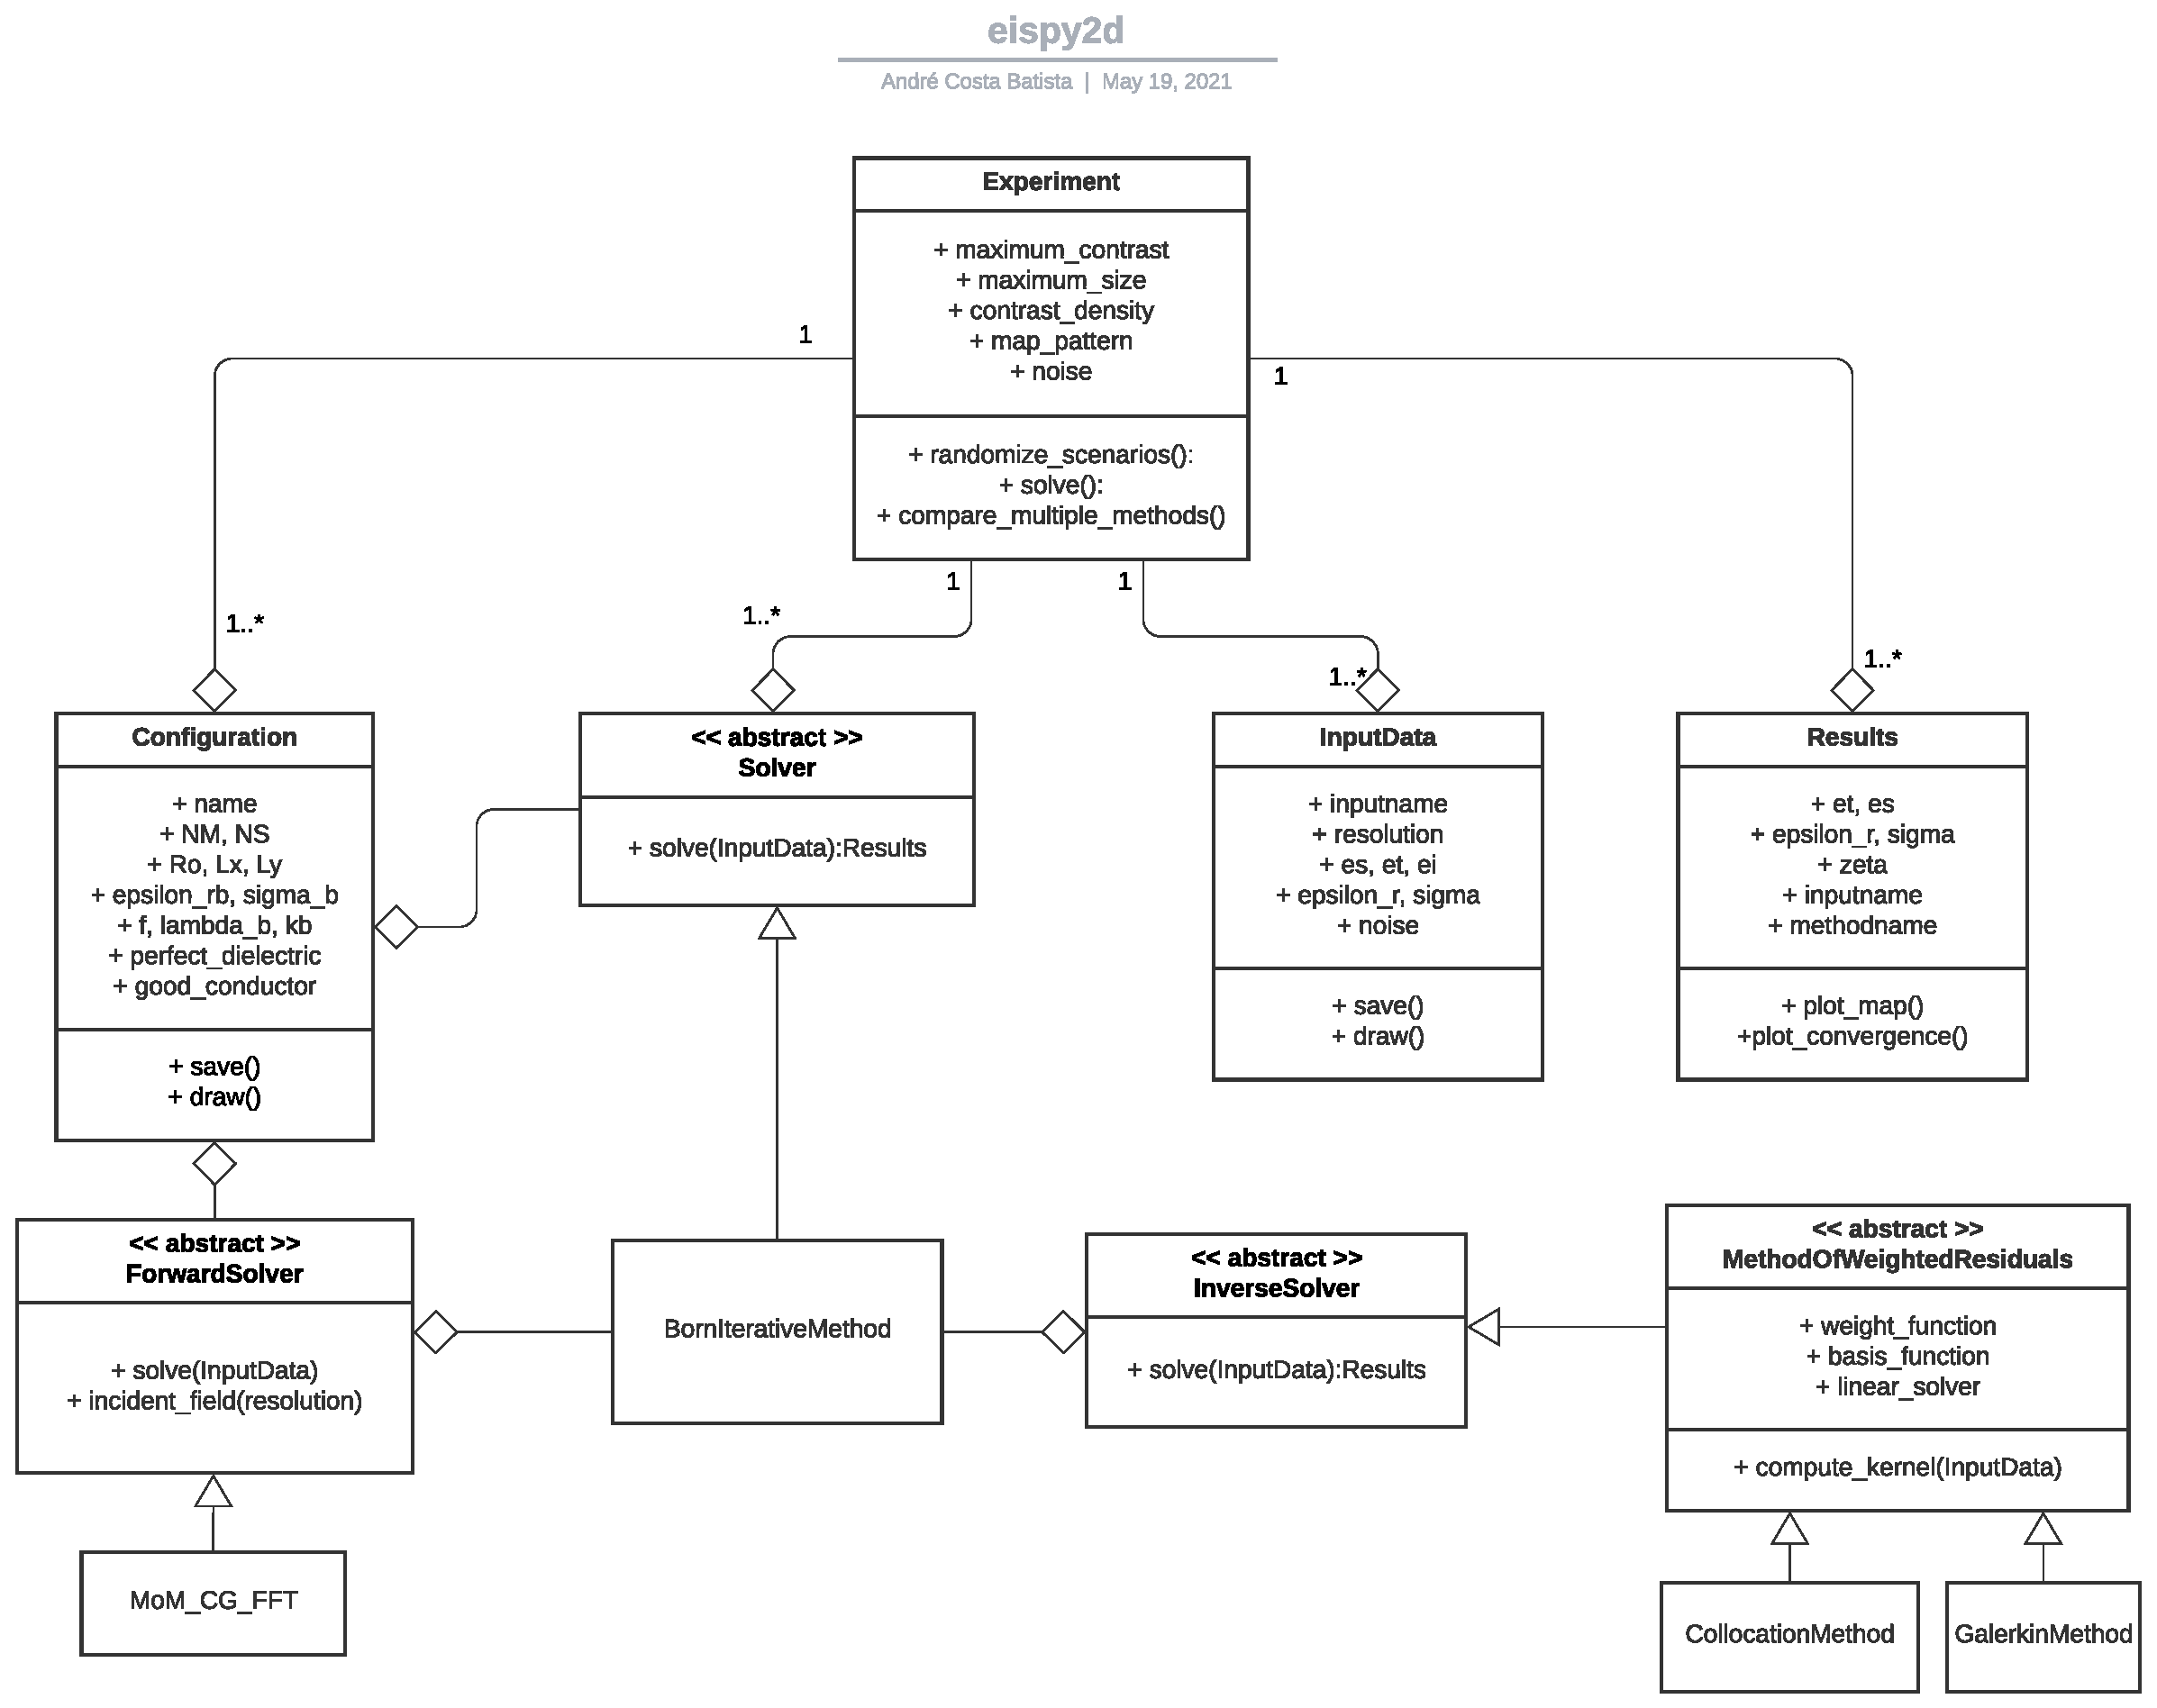
\includegraphics[width=.95\paperwidth, angle=90]{./figuras/eispy2d.eps}
				\vspace*{0.2in}
				\caption{UML Class Diagram of \textit{eispy2d} library.}
				\label{fig:4:eispy2d}
			\end{figure}
		
			%A seguir, uma breve explicação das classes principais:
			The following is a brief explanation of the main classes:
			\begin{enumerate}
				%\item\textbf{Configuration}: classe que guarda as informações principais do problema, como tamanho da imagem ($L_X$, $L_Y$), raio de observação ($R_O$), número de medições e de incidências ($N_M$, $N_S$);
				\item\textbf{Configuration}: a class that stores the primary information of the problem, such as image size ($L_X$, $L_Y$), observation radius ($R_O$), number of measurements and incidences ($N_M$, $N_S$);
				%\item\textbf{InputData}: classe que caracteriza uma instância de problema. Sua informação principal são os dados do campo espalhado. No entanto pode agregar outras informações como o campo total (para o problema linear) ou as imagens de contraste (para medição do erro);
				\item\textbf{InputData}: a class that characterizes a problem instance. Its primary information is the data of the scattered field. However, other information can be added, such as the total field (for the linear problem) or the contrast images (for error measurement);
				%\item\textbf{Results}: classe que guarda e exibe os resultados de uma execução do problema inverso não-linear. Além disso, também implementa os indicadores de qualidade;
				\item\textbf{Results}: a class that stores and displays the results of an execution of the nonlinear inverse problem. In addition, it also implements quality indicators;
				%\item\textbf{Solver}: uma classe abstrata para implementação de resolvedores do problema não-linear. Uma derivação, por exemplo, é a classe \textit{BornIterativeMethod} que implementa o correspondente método;
				\item\textbf{Solver}: a abstract class for nonlinear inverse solvers implementation. For instance, the class \textit{BornIterativeMethod}  is derived class that implements the corresponding method.
				%\item\textbf{ForwardSolver}: classe abstrata para implementação de resolvedores diretos. Uma derivação, por exemplo, é o Método dos Momentos (\textit{MoM\_CG\_FFT});
				\item\textbf{ForwardSolver}: abstract class for implementing forward solvers. One derivation, for example, is the Method of Moments (\textit{MoM\_CG\_FFT});
				%\item\textbf{InverseSolver}: classe abstrata para resolver o problema inverso linear. A classe \textit{MethodOfWeightedResiduals} é uma derivação ainda abstrata que serve para representar as discretizações \textit{CollocationMethod} e \textit{GalerkinMethod} e executar regularizadores como o de Tikhonov, Landweber e CG;
				\item\textbf{InverseSolver}: abstract class to solve the linear inverse problem. The \textit{MethodOfWeightedResiduals} class is a still abstract derivation that serves to represent the \textit{CollocationMethod} and \textit{GalerkinMethod} discretizations and execute regularizers such as Tikhonov, Landweber, and CG;
				%\item\textbf{Experiment}: classe que representa um experimento. É responsável por criar um conjunto de testes sintéticos aleatórios, executar os algoritmos e comparar resultados. Seus atributos principais são os parâmetros que configuram o conjunto de teste, i.e., o padrão de espalhado (geometrias tradicionais, aleatórias ou superfícies), o contraste máximo permitido, o tamanho máximo dos objetos, a densidade de contraste na imagem (quantidade de objetos na figura), entre outros.
				\item\textbf{Experiment}: a class that represents an experiment. It is responsible for creating a set of random synthetic tests, executing the algorithms, plotting results, and comparing results. Its main attributes are the parameters that configure the test set, i.e., the scatter pattern (traditional, random, or surface geometries), the maximum allowed contrast, the maximum size of the objects, the density of contrast in the image (number of objects in the image), among others.
			\end{enumerate}
			%Para avaliar ou comparar a performance entre os algoritmos, três aspectos são fundamentais: os indicadores de qualidade, os princípios para criação de conjuntos de teste aleatórios e a metodologia de comparação. As próximas subsubseções trarão maiores explicações destes três aspectos. Cada um deles incluem tanto técnicas já conhecidas quanto novas propostas implementadas neste trabalho que a contribuição desta investigação é uma estrutura mais robusta de experimentação sintética.
			Three aspects are fundamental to evaluate or compare the performance among the algorithms: the quality indicators, the principles for creating random test sets, and the comparison methodology. The following subsections will provide further explanations of these three aspects. Each of them includes both techniques already known and newly proposed ones; therefore, this investigation's contribution is a more robust structure of synthetic experimentation.
			
			\subsubsection{Performance Metrics Proposal}\label{chap:investigation:proposal:performance:metrics}
				
				%Um conjunto de indicadores foram implementados para a avaliar a qualidade da reconstrução feita pelos algoritmos. De maneira similar a \eqref{eq:4:error0:epsilon}, o erro percentual médio de estimação da permissividade relativa e o erro médio de estimação da condutividade serão calculados por:
				A set of indicators were implemented to assess the quality of the reconstruction done by the algorithms. Similar to \eqref{eq:4:error0:epsilon}, the average percentage error of estimation of relative permittivity and the average error of estimation of conductivity will be calculated by:
				\begin{align}
					\zeta_{\epsilon PAD} &= \frac{1}{N_IN_J}\sum\limits_{i=1}^{N_I}\sum\limits_{j=1}^{N_J}\left|\frac{\epsilon^*_{r,ij}-\epsilon_{r,ij}}{\epsilon^*_{r,ij}}\right|\times100~[\%] \label{eq:4:zeta:epad} \\
					\zeta_{\sigma AD} &= \frac{1}{N_IN_J}\sum\limits_{i=1}^{N_I}\sum\limits_{j=1}^{N_J}\left|\sigma^*_{ij}-\sigma_{ij}\right| \label{eq:4:zeta:sad}
				\end{align}
				
				%Além disso, foram implementados métricas similares a \eqref{eq:4:zeta:epad} e \eqref{eq:4:zeta:sad} mas que atuam particularmente sobre as regiões de fundo e de objeto. São eles:
				In addition, metrics similar to \eqref{eq:4:zeta:epad} and \eqref{eq:4:zeta:sad} were implemented, considering background and object regions only. They are:
				\begin{align}
					\zeta_{\epsilon BE} &= \frac{1}{N_B}\sum\limits_{\epsilon^*_{r,ij}=\epsilon_{rb}}^{N_I,NJ}\left|\frac{\epsilon^*_{r,ij}-\epsilon_{r,ij}}{\epsilon^*_{r,ij}}\right|\times100~[\%] \label{eq:4:zeta:ebe} \\
					\zeta_{\sigma BE} &= \frac{1}{N_B}\sum\limits_{\sigma^*_{ij}=\sigma_{b}}^{N_I,NJ}\left|\sigma^*_{ij}-\sigma_{ij}\right| \label{eq:4:zeta:sbe} \\
					\zeta_{\epsilon OE} &= \frac{1}{N_O}\sum\limits_{\epsilon^*_{r,ij}\neq\epsilon_{rb}}^{N_I,NJ}\left|\frac{\epsilon^*_{r,ij}-\epsilon_{r,ij}}{\epsilon^*_{r,ij}}\right|\times100~[\%] \label{eq:4:zeta:eoe} \\
					\zeta_{\sigma OE} &= \frac{1}{N_O}\sum\limits_{\sigma^*_{ij}\neq\sigma_{b}}^{N_I,NJ}\left|\sigma^*_{ij}-\sigma_{ij}\right| \label{eq:4:zeta:soe}
				\end{align}
				
				%\noindent onde $N_B$ e $N_O$ são o número elementos de fundo e de objeto, respectivamente. O objetivo dessas métricas é medir especificamente a capacidade de estimar o contraste de um objeto e de evitar perturbações nas regiões de fundo.
				\noindent where $N_B$ e $N_O$ are the numbers of background and object elements, respectively. The purpose of these metrics is to precisely measure the ability to estimate the contrast of an object and avoid perturbations in the background regions.
				
				%Em relação a EAs que otimizam simultâneamente contraste e campo, pode ser muito interessante medir a capacidade de estimar o campo total na região da imagem. Por isso, foram implementados os seguintes indicadores:
				Concerning EAs that simultaneously optimize contrast and field, measuring the ability to estimate the total field in the image region is a potential tool. For this reason, the following indicators were implemented:
				\begin{align}
					\zeta_{TFMPAD} &= \frac{1}{N_PN_QN_R}\sum\limits_{p=1}^{N_P}\sum\limits_{q=1}^{N_Q}\sum\limits_{r=1}^{N_R}\left|\frac{|E^*_{pqs}|-|E_{pqs}|}{|E^*_{pqs}|}\right|\times100~[\%] \label{eq:4:zeta:tfmpad} \\
					\zeta_{TFPAD} &= \frac{1}{N_PN_QN_R}\sum\limits_{p=1}^{N_P}\sum\limits_{q=1}^{N_Q}\sum\limits_{r=1}^{N_R}\left|\measuredangle E^*_{pqs} - \measuredangle E_{pqs}\right| \label{eq:4:zeta:tfpad}
				\end{align}
			
				%\noindent onde o operador ``$\measuredangle$'' representa a fase do número complexo. Portanto, esses dois indicam medem o erro médio de magnitude e fase da estimativa do campo elétrico.
				\noindent where the operator ``$\measuredangle$'' represents the phase of the complex number. Therefore, these two indicators measure the average magnitude and phase error of the electric field estimate.
				
				%Quando um algoritmo erra na localização e na detecção da forma dos objetos, as métricas \eqref{eq:4:zeta:epad}-\eqref{eq:4:zeta:soe} serão afetadas. No entanto, pode ser que um algoritmo estime bem a forma e o contraste de um objeto mas, por erros na posição, a avaliação dessa solução pelas métricas seja baixa. Para levar em conta especificamente a capacidade de detectar posição e forma, são propostas duas métricas.
				When an algorithm fails to locate and detect the shape of objects, metrics \eqref{eq:4:zeta:epad}-\eqref{eq:4:zeta:soe} will be affected. However, it may be that an algorithm estimates the shape and contrast of an object well, but due to errors in position, the evaluation of this solution by the metrics is low. Two metrics are proposed to take specific account of the ability to detect position and shape.
				
				%Para avaliar a capacidade de estimar a posição de objetos, é proposto um indicador baseado na distância entre os ``centros de massa'' dos objetos nas imagens:
				An indicator based on the distance between the ``centers of mass'' of the objects in the images is proposed to assess the ability to estimate the position of objects:
				\begin{equation}
					\zeta_P  = \sqrt{(x^*_c-x_c)^2 + (y^*_c-y_c)^2}\times 100~[\%] \label{eq:4:zeta:p}
				\end{equation}
			
				%\noindent onde ($x^*_c$, $y^*_c$) é centro da figura original e ($x_c$, $y_c$) é o centro da imagem reconstruída. Os centros são calculados conforme \autoref{alg:zetap}. Após a limiarização da imagem reconstruída, os valores de contraste são descartados. Isto é feito para evitar que erros na estimativa do contraste influenciem na ponderação do centro. Desta forma, esse indicador pode ser utilizado tanto para imagens com objetos únicos como múltiplos.
				\noindent where ($x^*_c$, $y^*_c$) is the center of the original figure and ($x_c$, $y_c$) is the center of the reconstructed image. The centers are calculated according to \autoref{alg:zetap}. After the threshold of the reconstructed image, the contrast values are discarded. This is done to prevent errors in the contrast estimation from influencing the center weighting. In this way, this indicator can be used for images with single or multiple objects.
				\begin{algorithm}[!htb]
					\caption{$\zeta_P$ measure.}
					\label{alg:zetap}
					\KwIn{$\boldsymbol{\chi^{*}}$, $\boldsymbol{\chi}$}
					\KwOut{$\zeta_P$}
					$\chi_{thres} \leftarrow \min\{|\boldsymbol{\chi}|\} + \frac{1}{2}\left(\max\{|\boldsymbol{\chi}|\}-\min\{|\boldsymbol{\chi}|\}\right)$\\
					$\chi^{*}_{ij}\leftarrow1~\forall\chi^{*}_{ij}\neq0$\\
					$\chi_{ij}\leftarrow\begin{cases} 0, &\forall\chi_{ij}<\chi_{thres} \\ 1, &\forall\chi_{ij}\ge\chi_{thres}\end{cases}$ \\
					$x_i \leftarrow (i-1)/(N_I-1) \forall i = 1, \cdots, N_I$\\
					$y_j \leftarrow (j-1)/(N_J-1) \forall j = 1, \cdots, N_J$\\
					$x^*_c\leftarrow \frac{\sum_{i=1}^{N_I}\sum_{j=1}^{N_J} x_i\chi^*_{ij}}{\sum_{i=1}^{N_I}\sum_{j=1}^{N_J}\chi^*_{ij}}$ \\
					$y^*_c\leftarrow \frac{\sum_{i=1}^{N_I}\sum_{j=1}^{N_J} y_j\chi^*_{ij}}{\sum_{i=1}^{N_I}\sum_{j=1}^{N_J}\chi^*_{ij}}$ \\
					$x_c\leftarrow \frac{\sum_{i=1}^{N_I}\sum_{j=1}^{N_J} x_i\chi_{ij}}{\sum_{i=1}^{N_I}\sum_{j=1}^{N_J}\chi_{ij}}$ \\
					$y_c\leftarrow \frac{\sum_{i=1}^{N_I}\sum_{j=1}^{N_J} y_j\chi_{ij}}{\sum_{i=1}^{N_I}\sum_{j=1}^{N_J}\chi_{ij}}$ \\
					$\zeta_P  = \sqrt{(x^*_c-x_c)^2 + (y^*_c-y_c)^2}\times 100~[\%]$
				\end{algorithm}
			
				%Para avaliar a capacidade de reconstruir a forma dos objetos, foi necessário utilizar um algoritmo de detecção de contornos nas imagens. O algoritmo Marching Cubes \citep{lorensen1987marching} é uma técnica clássica de identificação de contornos em imagens tridimensionais. A biblioteca \textit{scikit-image} possui uma implementação eficiente do caso dimensional que será utilizada nesse trabalho \citep{walt2014scikit}. A partir disso, a métrica de forma $\zeta_S$ é definida em termos da razão entre a área da diferença entre os contornos das duas imagens e a área da imagem original. A implementação e um exemplo para o cálculo desta métrica pode ser visualizada no Anexo \ref{annex:zetas}. Tanto $\zeta_S$ quanto $\zeta_P$ são indicadores que não existem ainda na literatura e estão sendo propostas nesse trabalho. Também não foi visto na literatura indicadores como $\zeta_{TFMPAD}$ e $\zeta_{TFPAD}$. Embora eles não tenham tanta relevância por não ser o objetivo principal reconstruir o campo, eles podem auxiliar no entendimento do desempenho dos métodos, principalmente dos estocásticos que otimizam simultâneamente contraste e campo.
				It was necessary to use an algorithm for detecting contours in the images to assess the ability to reconstruct the shape of the objects. The Marching Cubes algorithm \citep{lorensen1987marching} is a classic technique for identifying contours in three-dimensional images. The \textit{scikit-image} library efficiently implements the two-dimensional case, which is considered in this work \citep{walt2014scikit}. Then, the shape metric $\zeta_S$ is defined in terms of the ratio between two areas: (i) the area of the difference between the contours of the two images; and (ii) the area of the original image. The implementation and an example for calculating this metric can be seen in Appendix \ref{annex:zetas}. This approach is not as sophisticated as the one proposed by \cite{kurrant2021evaluating}. Our approach is based on a threshold technique which is not as robust as an image segmentation through a machine learning technique. In addition, their diverse set of metrics for breast reconstruction can also be adapted to our general scheme and it will be consider in the future. However, as far as this author knows, both $\zeta_S$ and $\zeta_{P}$ are indicators that have not been addressed in general reconstructions. Also, indicators such as $\zeta_{TFMPAD}$ and $\zeta_{TFPAD}$ were not seen in the literature. Although they are not so relevant because it is not the primary objective to reconstruct the field, they can help understand the performance of methods, especially the stochastics that simultaneously optimize contrast and field.
				
			\subsubsection{Randomization of the Test Set}\label{chap:investigation:proposal:performance:randomization}
			
				%Em muitos trabalhos, os experimentos sintéticos são planejados para demonstrar a capacidade de reconstrução dos algoritmos em cenários variados. Tradicionalmente, geometrias comuns são utilizadas para explorar situações como presença de espalhadores fortes, diferentes níveis de ruído, separação de objetos, heterogeneidades, entre outros. Normalmente, as imagens utilizadas nos testes são definidas arbitrariamente e a performance em tipo de situação é estudada com apenas um ou poucos exemplos de imagens.
				In many studies, synthetic experiments are designed to demonstrate the ability to reconstruct the algorithms in different scenarios. Traditionally, common geometries are used to explore situations such as strong scatterers, different noise levels, separation of objects, heterogeneities, among others. Usually, the images used in the tests are defined arbitrarily, and the performance in the corresponding situation is studied with only one or a few examples of images.
				
				%Para dar alguns exemplos, citaremos alguns trabalhos recentes e relevantes na literatura: (i) \cite{zhong2020multiresolution} utilizaram um tipo de imagem pra fazer comparações entre quatro níveis de ruído e um tipo de imagem para compara situação de alto contraste; (ii) \cite{wei2019deep} usam quatro imagens para cada um dos dois níveis de contraste e três imagens para estudar a reconstrução de objetos condutivos; e (iii) \cite{salucci2017multifrequency} usou uma imagem para testes sem ruído, uma imagem para dois níveis de ruído, uma imagem para não-homogeneidade e uma imagem para alto contraste. Nestes trabalhos, vale destacar que as imagens ou são compostas por somente círculos ou único quadrado ou o tradicional perfil Austria (composto por um anel e dois círculos). No entanto, vale destacar também que, em \citep{wei2019deep}, os autores utilizaram seis imagens de uma base formada por handwritng digits comumente usada em Machine Learning; em \citep{shah2018fast} e \citep{batista2021quadratic}, os autores usam quatro imagens com geometrias diferentes para experimentos com objetos únicos e três para não-homogeneidades com diferentes geometrias.
				To give some examples, we will mention some recent and relevant works in the literature: (i) \cite{zhong2020multiresolution} used an image type to make comparisons between four noise levels and an image type to compare high contrast situations; (ii) \cite{wei2019deep} use four images for each of the two levels of contrast and three images to study the reconstruction of conductive objects; and (iii) \cite{salucci2017multifrequency} used an image for tests without noise, an image for two levels of noise, an image for inhomogeneity and an image for high contrast. In these works, it is worth mentioning that the images are either composed of only circles or a single square or the traditional Austria profile (composed of a ring and two circles). However, it is also worth noting that, in \citep{wei2019deep}, the authors used six images of a base formed by handwritng digits commonly used in Machine Learning; in \citep{shah2018fast} and \citep{batista2021quadratic}, the authors use four images with different geometries for experiments with single objects and three for inhomogeneities with different geometries.
				
				%De fato, o estilo de experimentação que é tradicionalmente usado exemplifica a capacidade do algoritmo de lidar com diferentes situações e isso é relevante para a testagem do método. No entanto, não seria mais robusto avaliar a performance com experimentos sintéticos através um conjunto suficientemente grande de imagens com geometrias aleatórias? Não seria esse um procedimento mais robusto para estudar a performance média dos algoritmos? A performance média em conjuntos de teste aleatórios não seria melhor do que o estudo com imagens arbitrárias para fazer uma comparação mais eficiente? Esse tipo de estudo não seria relevante para a literatura tal como já é na área de comparação de algoritmos de otimização \citep{beiranvand2017best}?
				In fact, the form of experimentation traditionally used exemplifies the algorithm's ability to deal with different situations, which is relevant for testing the method. However, wouldn't it be more robust to evaluate performance with synthetic experiments through a sufficiently large set of images with random geometries? Wouldn't this be a more robust procedure to study the average performance of the algorithms? Wouldn't the average performance in random test sets be better than the study with arbitrary images to make a more efficient comparison? Wouldn't this type of study be relevant to the literature as it is already in the comparison of optimization algorithms \citep{beiranvand2017best}?
				
				%Para explorar esse tipo de experimentação, foi desenvolvido um processo de geração de conjunto de testes aleatórios dentro da classe \textit{Experiment} na biblioteca \textit{eispy2d}. Um conjunto de testes é gerado conforme os seguintes parâmetros de configuração:
				A process of generating a set of random tests was developed to explore this experimentation design. It is embedded within the \textit{Experiment} class in the \textit{eispy2d} library. A set of tests is generated according to the following configuration parameters:
				\begin{itemize}
					%\item Padrão de geometrias: esse parâmetro significa que tipo de geometrias serão consideradas. Três padrões foram implementados: geometrias regulares\footnote{Quadrado, retângulo, triângulo equilátero, cruz, círculo, anel, elipse, losângulo, trapézio, paralelograma, polígonos de mais 5 lados (pentágono, hexágono etc) e estrelas de 4, 5 e 6 pontas.}, polígonos aleatórios\footnote{Polígonos de 3 lados ou mais com raio entre centro e vérticos aleatórios.} e superfícies aleatórias\footnote{Somatório de senos ou exponenciais}.
					\item Geometry pattern: this parameter means what type of geometries will be considered. Three patterns were implemented: regular geometries\footnote{Square, rectangle, equilateral triangle, cross, circle, ring, ellipse, rhombus, trapezoid, parallelogram, polygons of more than five sides (pentagon, hexagon, etc.) and stars of 4, 5, and 6 points.}, random polygons\footnote{Polygons of 3 sides or more with random radius between the center and vertices.}, and random surfaces\footnote{Sum of sines or exponentials.}.
					%\item Máximo contraste: esse parâmetro controla o intervalo de contraste permitido para os objetos inseridos na imagem. Também é possível configurar esse parâmetro para que todos os objetos sejam definidos com esse contraste. Ou seja, o conjunto de testes pode ser criado tanto para estudar o desempenho com diferentes contrastes quanto únicos.
					\item Maximum contrast: this parameter controls the allowed contrast range for the objects inserted in the image. It is also possible to configure this parameter so that all objects are defined with this contrast. In other words, the set of tests can be created both to study performance with different and unique contrasts.
					%\item Máximo tamanho: esse parâmetro regula o tamanho dos objetos. Também pode ser definido como valor máximo ou configurado para valor fixo. No caso de geometrias regulares, todas elas são configuradas para que o raio entre o centro e o vértice mais afastado seja definido por esse parâmetro. Em outras palavras, é o maior desenho da geometria que cabe dentro de um círculo definido por esse parâmetro. No caso de polígonos aleatórios, esse parâmetro regula o raio máximo que cada vértice pode ter. No caso de exponenciais, esse parâmetro regula o raio máximo do centro da exponencial até três vezes o desvio padrão.
					\item Maximum size: this parameter regulates the size of objects. It can also be set to a maximum value or assigned to a fixed value. In regular geometries, all of them are configured so that this parameter defines the radius between the center and the furthest vertex (see Appendix \ref{annex:geometries} for more information). In other words, it is the largest geometry drawing that fits within a circle defined by this parameter. In the case of random polygons, this parameter regulates the maximum radius that each vertex can have. In exponentials, this parameter controls the maximum radius of the exponential up to three times the standard deviation.
					%\item Máxima densidade de contraste: regula o valor máximo da média de contraste por píxel da imagem. Esse parâmetro regula a quantidade de objetos na imagem.
					\item Maximum contrast density: regulates the maximum value of the average contrast per pixel of the image. This parameter regulates the number of objects in the image.
					%\item Ruído: nível de ruído no qual os dados do campo espalhado vão ser corrompidos.
					\item Noise: noise level at which the data in the scattered field will be corrupted.
					%\item Tamanho amostral: quantidade de imagens de teste no conjunto.
					\item Sample size: number of test images in the set.
				\end{itemize}
				%É importante destacar que cada geometria inserida em uma imagem tem rotação e posição definidas aleatoriamente. Portanto, o objetivo deste processo é criar benchmarks que possibilitem o estudo da performance do métodos sejam em configurações isoladas mas também na evolução de efeitos (e.g., a evolução da performance no crescimento do contraste). Não somente isso, esse processo permite estudar fatores de efeito na performance dos algoritmos para o problema isolando o viés presente na escolha arbitrária das geometrias. Essa implementação considera apenas experimentos sintéticos. No entanto, esses princípios poderiam ser utilizados para um projeto de um benchmark real, i.e., medições reais de espalhamentos os quais são definidos seguindo esses princípios de aleatorização de geometrias e isolamente de fatores de efeito.
				It is important to highlight that each geometry inserted in an image has a randomly defined rotation and position. Therefore, this process aims to create benchmarks that make it possible to study the performance of the methods in isolated configurations and the evolution of effects (e.g., the progression of performance in the growth of the contrast). Not only that, this process allows the study of effect factors on the performance of the algorithms for the problem, isolating the bias present in the arbitrary choice of geometries. This implementation considers only synthetic experiments. However, these principles could be used for a project of a real benchmark, i.e., physical measurements, which are defined following these principles of randomization of geometries and in isolation of effect factors.

			\subsubsection{Comparison Structure}\label{chap:investigation:proposal:performance:comparison}
				
				%Quando um método é executado para um conjunto de testes, o indicador de performance é calculado para solução final de cada instância do conjunto. A informação dos resultados pode ser visualizada de diferentes formas. Duas das formais mais tradicionais para visualizar os dados de uma amostra é o \textit{boxplot} e o \textit{violinplot} \citep{chen2008handbook}. A primeira é importante para visualizar os quantis de uma amostra e a última é importante para ter uma noção da distribuição dos dados. Rotinas para visualização dos dados dos experimentos através desses dois gráficos foram implementadas a partir da biblioteca \textit{matplotlib} \citep{hunter2007matplotlib}. Além disso, as rotinas também implementam a visualização de mais de um conjunto de teste em um mesmo gráfico o qual é relevante para visualizar a evolução da performance de um método quando se varia algum parâmetro na configuração dos testes (e.g., contraste máximo). Também foi utilizado o gráfico Quantile-Quantile para verificação de premissas de normalidade de distribuição implementados pela rotina \textit{qqplot} da biblioteca \textit{pingouin} \citep{vallat2018pingouin}.
				When a method runs a set of tests, the performance indicator is calculated for the final solution of each instance. The results information can be viewed in different ways. Two of the most traditional ways to visualize the data of a sample are the \textit{boxplot} and the \textit{violinplot} \citep{chen2008handbook}. The first is essential to visualize the quartiles of a sample, and the last is important to get a sense of the distribution of the data. Routines for visualizing the data of the experiments through these two graphs were implemented from the \textit{matplotlib} library \citep{hunter2007matplotlib}. In addition, the routines also implement the visualization of more than one test set in the same graph, which is relevant to visualize the evolution of the performance of a method when a parameter in the test configuration varies (e.g., maximum contrast). The Quantile-Quantile graph was also used to verify assumptions of normality distribution implemented by the \textit{qqplot} routine of the \textit{pingouin} library \citep{vallat2018pingouin}.
				
				%Os conjuntos de teste representam uma amostra de um universo de casos possíveis. A informação da performance média de método em um universo particular pode ser relevante tanto para cumprir especificações numa dada aplicação quanto para comparação com outras metodologias. Como esse universo de casos é muito grando, se não infinito, é muito comum estimar o intervalo de confiança dessa média, i.e., uma faixa de valores que têm uma alta probabilidade de conter a média verdadeira. Este tipo de estudo é feito utilizando ferramentas estatísticas que possibilitam não somente estimar a média como também comparar outras, ou seja, fazer comparações entre performances médias de algoritmos ou conjuntos de teste. Não está no escopo desta dissertação uma explicação sobre os métodos estatísticos que foram utilizados. Para uma melhor compreensão, recomendamos a leitura de \citep{montgomery2010applied} e as implementações da biblioteca \textit{statsmodels} \citep{seabold2010statsmodels}. Neste texto será somente apresentado o processo de comparação entre duas e múltiplas amostras as quais representam os resultados de um indicador para diferentes métodos em um mesmo conjunto de testes.
				The test sets represent a sample of a universe of possible cases. The information on the average performance of the method in a particular universe can be relevant to comply with specifications in a given application and for comparison with other methodologies. As this universe of cases is very large, if not infinite, it is common to estimate the confidence interval of this average. The confidence interval can be understood as the range in which, if we repeat the experiment many times, the sampled average will be within that range in a specified percentage of the number of times. This type of study is done using statistical tools that make it possible to estimate the average and compare others, that is, to make comparisons between average performances of algorithms or test sets. It is not in the scope of this dissertation to explain the statistical methods that were used. We recommend the reading of \citep{montgomery2010applied} and the implementations of the \textit{statsmodels} library \citep{seabold2010statsmodels} for a better understanding. In this text, only the comparison process between two and multiple samples will be presented, representing the results of an indicator for different methods in the same set of tests.
				
				%O processo de comparação da perfomance de um indicador entre dois métodos em para um mesmo conjunto de teste foi implementado segundo uma lógica pareada. Uma vez que se trata dos resultados dos métodos para um mesmo conjunto de teste, a média estimada é definida em termos da diferença entre indicadores dos dois métodos em cada instância. O processo pode ser resumido da seguinte forma:
				The process of comparing the performance of an indicator between two methods in the same test set was implemented according to a paired fashion. Through the results of the methods for the same test set, the estimated average is defined in terms of the difference between indicators of the two methods in each instance.  The process can be summarized as follows:
				\begin{enumerate}
					%\item Se o teste de Shapiro-Wilk não acusar um desvio da normalidade sobre a diferença pareada, então o Teste T-Pareado com significância de 5\% é realizado e o tamanho de efeito\footnote{O tamanho de efeito neste caso significa a diferença mínima pareada para o qual é possível indentificar um erro de falso-negativo para a potência desejada e tamanho amostral, i.e., quando a hipótese de iguadade não é reijeitada quando é falsa.} é calculado para uma potência de 80\%. Se for detectada uma diferença, então haverá evidência para a superioridade de um dos métodos.
					\item If the Shapiro-Wilk test does not show a deviation from normality over the paired difference, then the Paired T-Test with a significance of 5\% is performed. The effect size\footnote{The effect size, in this case, means the minimum paired difference for which it is possible to identify a false-negative error for the desired power and sample size, i.e., when the hypothesis of equality is not rejected when it is false.} is calculated for a power of 80\%. If a difference is detected, then there is evidence for the superiority of one of the methods.
					%\item Se o teste de Shapiro-Wilk acusar um desvio da normalidada sobre a diferença pareada, então o teste é repetido utilizando transformações logarítmicas e de raiz quadrada sobre os dados. Se uma transformação tiver sucesso, então o mesmo procedimento do passo anterior é repetido e as mesmas conclusões podem ser obtidas.
					\item If the Shapiro-Wilk test shows a deviation from the normal distribution over the paired difference, then the test is repeated using logarithmic and square-root transformations on the data. If a transformation is successful, then the same procedure as the previous step is repeated, and the same conclusions can be drawn.
					%\item Se nenhuma das transformações tiver sucesso, então é realizado o Teste de Wilcoxon que permite detectar as diferenças seguem uma distribuição simétrica ao redor de zero. Se a diferença for detectada a um nível de significância de 5\%, então haverá evidência para a superioridade de um dos métodos.
					\item If none of the transformations are successful, then the Wilcoxon Test is performed, which allows the detection of differences following a symmetrical distribution around zero. If the difference is detected at a significance level of 5\%, then there is evidence for the superiority of one of the methods.
				\end{enumerate}
				%As premissas de independência entre os dados são garantidas pelo fato da independência das execuções dos algoritmos. As rotinas utilizadas para o teste normal são as da biblioteca \textit{statsmodels} e a rotina do teste não-normal provém da biblioteca \textit{scipy} \citep{scipy}.
				The assumptions of independence between the data are guaranteed because the algorithms' execution is independent. When the normality assumption is valid, the routines used are those in the \textit{statsmodels} library, and the non-normal test routine comes from the \textit{scipy} library \citep{scipy}.
				
				%O processo de comparação entre múltiplos métodos se dá pela técnica de Análise de Variâncias (ANOVA) \citep{montgomery2010applied}. O processo de comparação se dá através da seguinte forma:
				The comparison process between multiple methods takes place using the analysis of variances (ANOVA) \citep{montgomery2010applied}. The comparison process is described as follows:
				\begin{enumerate}
					%\item Os resíduos de cada amostra em relação às suas médias amostrais são calculadas.
					\item The residues of observations and their corresponding sample means are evaluated.
					%\item Se o Teste de Shapiro-Wilk não acusar um desvio da distribuição dos resíduos, seja sem ou com transformações:
					\item If the Shapiro-Wilk test does not indicate a deviation between residuals and normal distributions, either with or without transformations:
					\begin{enumerate}
						%\item Se o Teste de Fligner não acusar invalidade da condição de homocedasticidade\footnote{A condição de homocedasticidade significa igualdade de variâncias das amostras.}, então o One Way ANOVA é executado sob o nível de significância de 5\%. O resultado indicará se existe evidência para pelo menos uma performance diferente das demais ou não. Também é calculado o tamanho de efeito para uma potência de 80\%.
						\item If the Fligner Test does not indicate invalidity of the homoscedasticity assumption\footnote{The homoscedasticity assumption means equal sample variances.}, then the One Way ANOVA is performed under the 5\% significance level. The result will indicate whether there is evidence for at least one performance different from the others or not. The effect size is also calculated for a power of 80\%.
						%\item Se o Teste de Fligner acusar invalidade da premissa de homocedasticidade, então é executado o teste Welch ANOVA o qual poderá indicar evidência para pelo menos uma performance diferente das demais sob um nível de significância de 5\%.
						\item If the Fligner test reveals invalidity of the homoscedasticity premise, then the Welch ANOVA test is performed, which may indicate evidence for at least one performance different from the others under a 5\% significance level.
						%\item Se for detectada alguma diferença e for necessário tentar identificar todas as possíveis superioridades de performance:
						\item If any differences are detected and it is necessary to try to identify all possible performance superiorities:
						\begin{enumerate}
							%\item Se a condição de homocedasticidade for válida, será realizado o Teste Tukey HSD de Comparações Múltiplas e serão detectadas todas as diferenças com a correção de significância necessária.
							\item If the homoscedasticity assumption is valid, the Tukey HSD Multiple Comparison Test will be performed and all differences will be detected with the necessary significance correction.
							%\item Se a condição de homocedasticidade não for válida, então as múltiplas comparações serão feitas a partir de múltiplos teste de Welch para amostras independentes com a significância determinada pela correção de Bon-Ferroni.
							\item If the homoscedasticity condition is not valid, multiple comparisons will be made from multiple Welch T tests for independent samples with the significance determined by the Bon-Ferroni correction.
						\end{enumerate}
						%\item Se for detectada alguma diferença e for necessário identificar somente se um dos métodos é superior ou inferior aos outros:
						\item If a difference is detected and it is necessary to identify if all methods are superior or inferior to a single one (all versus one):
						\begin{enumerate}
							%\item Se a condição de homocedasticidade for válida, será realizado o Teste de Dunnet com a correção de significância necessária.
							\item If the homoscedasticity condition is valid, the Dunnet Test will be performed with the necessary significance correction.
							%\item Se a condição de homocedasticidade não for válida, então as comparações serão feitas a partir de teste de Welch para amostras independentes com a significância determinada pela correção de Bon-Ferroni.
							\item If the homoscedasticity premise is not valid, then the comparisons will be made using the Welch test for independent samples with the significance determined by the Bon-Ferroni correction.
						\end{enumerate}
					\end{enumerate}
					%\item Se não for possível assumir a normalidade dos resíduos, então será realizado o Teste de Kruskal-Wallis com um nível de significância de 5\% que permite identificar se pelo menos uma das amostras veio de uma distribuição diferente de qualquer outra.
					\item If it is not possible to assume the normality of the residues, then the Kruskal-Wallis test will be performed with a significance level of 5\%. The test allows identifying whether at least one of the samples came from a different distribution from any other.
					\begin{enumerate}
						%\item Se for detectada qualquer diferença e for necessária identificar todas possíveis, então são realizados múltiplos testes U de Mann-Whitney. Este teste permite identificar se existe evidência para uma probabilidade maior que 50\% para superioridade de algum dos dois métodos.
						\item If any difference is detected and it is necessary to identify all possible ones, then multiple Mann-Whitney U tests are performed. This test makes it possible to identify whether there is evidence for a probability greater than 50\% for the superiority of either method.
						%\item Se for detectada qualquer diferença e for necessária identificar apenas se um método é superior a outro, então são realizados testes U de Mann-Whitney para fazer as comparações necessárias.
						\item If any difference is detected and it is necessary to identify only if one method is superior to another, then Mann-Whitney U tests are performed to make the necessary comparisons.
					\end{enumerate}
				\end{enumerate}
				%Assim como no processo anterior, a hipótese de independência de observações é garantida pelo processo de execução dos algoritmos. As implementações do testes para dados normais são os disponíveis na biblioteca \textit{statsmodels} e, os não-normais, na \textit{scipy}.
				As in the previous process, the hypothesis of independence of observations is guaranteed by the process of executing the algorithms. Test implementations for normal data are those available in the \textit{statsmodels} library and non-normal ones in \textit{scipy}.
				
				%Por fim, também foi implementada a técnica Análise Fatorial para dois e três fatores, conforme descrita no capítulo 14 de \citep{montgomery2010applied}. Esta técnica é utilizada para identificar tanto se um fator de efeito tem impacto na performance de um algoritmo como a interação desse fator com outros dois. Por exemplo, através desse tipo de análise é possível identificar se o aumento do tamanho e da quantidade de objetos na imagem influencia em sua performance assim como identificar se a variação desses dois fatores ao mesmo tempo tem algum impacto. A análise foi padronizada para um nível de significância de 5\% e a premissas de normalidade e homocedasticidade são verificadas pelos teste de Shapiro-Wilk e Fligner.
				Finally, the Factor Analysis technique for two and three factors was also implemented, as described in chapter 14 of \citep{montgomery2010applied}. This technique is used to identify both if an effect factor impacts the performance of an algorithm and the interaction of that factor with more others. For example, through this type of analysis, it is possible to identify whether the increase in the size and number of objects in the image influences its performance as well as to identify whether the variation of these two factors at the same time has any impact. The analysis was standardized to a significance level of 5\% and the normality and homoscedasticity assumptions are verified by the Shapiro-Wilk and Fligner tests.


		\subsection{State-of-Art EAs for EISP}\label{chap:investigation:proposal:stateofart}
			
			%Além das formulações tradicionais de EAs, tais como o GA, DE, SA, ACO e o PSO, existem outras que tem sido desenvolvidas as quais são consideradas formulações ou técnicas do estado-da-arte de EAs. Uma delas são os Algoritmos Evolucionários Distribuídos (DEAs) que cuja a ideia principal é dividir a população em subpopulações, também chamadas de ilhas, com regras de trocas de informação \citep{gong2015distributed}. Esses algoritmos podem contribuir para um bom balanceamento entre exploration (busca global) e exploitation (busca local) o qual é importante para a qualidade da convergência e da preservação da diversidade. Estes dois aspectos são bem importantes para problemas com múltiplos mínimos e de larga escala.
			In addition to traditional formulations of EAs, such as GA, DE, SA, ACO, and PSO, others have been developed, which are considered state-of-the-art formulations or techniques. One of them is the Distributed Evolutionary Algorithms (DEAs), whose main idea is to divide the population into subpopulations, also called islands, with rules for exchanging information \citep{gong2015distributed}. These algorithms can contribute to a good balance between exploration (global search) and exploitation (local search), essential for convergence and diversity preservation. These two aspects are very important for problems with multiple minima and large-scale optimization.
			
			%Semelhantes aos DEAs, os Algoritmos Co-Evolucionários Cooperativos (CCEAs) são técnicas baseadas na decomposição do problema em subproblemas, cada um resolvido por uma ilha diferente com suporte de mecanismos de colaboração entre elas \citep{ma2019survey}. A inspiração dos CCEAs são os processos ecológicos de mutualismo onde diferentes espécies convivem através de relações benéficas mútuas. No entanto, ela é muito similar a uma estratégia ``dividir-pra-conquistar''. Esse tipo de algoritmo tem recebido bastante atenção dentro da literatura sobre EC.
			Similar to DEAs, Co-Evolutionary Cooperative Algorithms (CCEAs) are techniques based on decomposing the problem into subproblems, each solved by a different island with the support of collaboration mechanisms among them \citep{ma2019survey}. The inspiration of the CCEAs is the ecological processes of mutualism where different species coexist through mutually beneficial relationships. However, it is very similar to a ``divide-to-conquer'' strategy. This type of algorithm has received much attention in the literature on EC.
			
			%Além disso, competições da IEEE Congress on Evolutionary Computation (CEC), como a de otimização mono-objetivo e a otimização global em larga escala estimulam o desenvolvimento de EAs mais eficientes \citep{molina2018shade,li2019differential,sun2019decomposition}. Um destes algoritmos é o L-SHADE (Linear Population Size Reduction Success-History based Adaptive Differential Evolution) \citep{tanabe2014improving}. Baseado no mecanismo do DE, o L-SHADE implementa duas estratégias principais: (i) um mecanismo de adaptação dos parâmetros de cruzamento e mutação baseado numa arquivo de valores promissores; e (ii) redução linear do número de indivíduos na população longo das gerações.
			In addition, IEEE Congress on Evolutionary Computation (CEC) competitions, such as mono-objective optimization and large-scale global optimization, stimulate the development of more efficient EAs \citep{molina2018shade,li2019differential,sun2019decomposition}. One of these algorithms is the L-SHADE (Linear Population Size Reduction Success-History based Adaptive Differential Evolution) \citep{tanabe2014improving}. Based on the DE mechanism, L-SHADE implements two main strategies: (i) a mechanism for adapting the crossing and mutation parameters based on a file of promising values; and (ii) linear reduction in the number of individuals in the population over generations.
			
			%Como foi anunciado anteriormente, esta parte da investigação se propõe a explorar a aplicação de técnicas do estado-da-arte de EC no contexto de EISP, aproximando essas duas áreas de pesquisas. Essa investigação é pertinente para as duas áreas uma vez que, em primeiro lugar, o EISP representa um exemplo relevante de problema de larga escala o qual é um desafio atual em EC; e em segundo lugar, o avanço na performance de EAs em EISP pode ser muito importante para a viabilidade da sua aplicação em casos maiores, i.e., altas resoluções e problemas tridimensionais. Nestas situações, EAs podem ser muito relevantes uma vez que podem ser construídos sem o uso de operações caras como resolvedores diretos e decomposição de matrizes. Embora o alto número de variáveis represente uma dificuldade considerável para a convergência desses métodos, sua capacidade de abordar problemas com múltiplos mínimos é muito atraente e justifica o desafio de contornar as dificuldades.
			As previously announced, this part of the investigation aims to explore the application of state-of-the-art EC techniques in the context of EISP, bringing these two areas of research closer together. This investigation is relevant to both areas since, first, the EISP represents a relevant example of a large-scale problem which is a current challenge in EC. Second, the advancement in the performance of EAs in EISP can be significant for the feasibility of its application in large-scale cases, i.e., high resolutions and three-dimensional problems. EAs can be very relevant in these situations since they can be built without using expensive operations like direct resolvers and matrix decomposition. Although the high number of variables represents a considerable difficulty for the convergence of these methods, their ability to address problems with multiple minimums is very attractive and justifies the challenge of circumventing the difficulties.
			
			%Por isso, o objetivo é investigar se alguma dessas técnicas mais avançadas em EC podem trazer avanços na performance dos métodos estocásticos de EISP, particularmente nas formulações mais difíceis onde contraste e campo são otimizados simultâneamente. Embora a aplicação no problema tridimensional seja mais atraente, essa investigação contemplará somente o caso bidimensional. Essa escolha foi feita pelo motivo de concentrar esforços primeiramente no desenvolvimento de ideias, i.e., investigar as ideias em um caso mais simples para que, em pesquisas futuras, essas ideias sejam aplicadas em situações mais complexas, como o caso tridimensional. A contribuição dessa investigação não é comprometida com isso, uma vez que a investigação dessas ideias nessas metodologias representam uma novidade para a literatura de imageamento em microondas.
			Therefore, the objective is to investigate if any of these more advanced techniques in EC can bring advances in the performance of the stochastic methods of EISP, particularly in the most challenging formulations where contrast and field are optimized simultaneously. Although the application in the three-dimensional problem is more attractive, this investigation will only consider the two-dimensional case. This choice was made for the purpose of concentrating efforts primarily on the development of ideas, i.e., investigating the ideas in a more straightforward case so that, in future research, these ideas are applied in more complex situations, such as the three-dimensional case. The contribution of this investigation is not compromised with this since the investigation of these ideas in these methodologies represents a novelty for the microwave imaging literature.
			
			%As seguintes perguntas gerais nortearão a condução desta investigação: existe alguma superioridade na perfomance do L-SHADE em comparação com os algoritmos tradicionalmente empregados na literatura de EISP, i.e., PSO, GA e DE? Existe alguma diferença na perfomance do IMSA quando este é acoplado ao L-SHADE ao invés do PSO, como proposto por \cite{salucci2017multifrequency}? Existe alguma forma de distribuição do algoritmo em ilhas e comunicação entre elas (DEA) que é capaz de impactar positivamente a performance de um EA? Existe alguma forma de decompor o problema que permita a implementação de um CCEA? Se sim, isso traria algum impacto da performance?
			The following general questions will guide the conduct of this investigation: is there any superiority in the performance of L-SHADE compared to the algorithms traditionally used in the EISP literature, i.e., PSO, GA, and DE? Is there any difference in the performance of IMSA when it is coupled to L-SHADE instead of PSO, as proposed by \cite{salucci2017multifrequency}? Is there any form of island distribution and communication (DEA) that can positively impact an EA's performance? Is there any way to decompose the problem that allows the implementation of a CCEA? If so, would that have any performance impact?
			
			%Até o momento só foi possível implementar os seguintes algoritmos: PSO, GA, DE, L-SHADE, IMSA-PSO, IMSA-DE e IMSA-L-SHADE. Ainda não foi possível ainda abordar DEAs e CCEAs. Por isso, essa dissertação só discutirá estrutura e resultados preliminares das implementações realizadas. No entanto, a abordagem de DEAs e CCEAs está prevista para o terceiro e quarto ano de doutorado.
			So far, it has only been possible to implement the following algorithms: PSO, GA, DE, L-SHADE, IMSA-PSO, IMSA-DE, and IMSA-L-SHADE. It has not yet been possible to address DEAs and CCEAs. For this reason, this dissertation will only discuss the structure and preliminary results of the implemented algorithms. However, DEAs and CCEAs are planned for the third and fourth year of the doctorate.
			
			%Este capítulo não foi escrito com objetivo de detalhar o funcionamento dos algoritmos implementados, seja na forma tópicos enumerados, diagramas ou pseudocódigos. Embora isso seja importante para a qualidade da futura tese, julgamos que nesse momento seria mais importante somente anunciar os algoritmos utilizados uma vez que nessa investigação não existe nenhuma novidade em relação a eles. Portanto, no futuro será escrito um apêndice dedicado a esse assunto e por enquanto deixamos indicados as referências que discutem a estrutura desses algoritmos\footnote{Embora essas referências já foram citadas anteriormente, repetiremos aqui para fins de disponibilizar um lugar onde elas estão todas juntas: PSO, GA, DE \citep{eiben2015introduction,gaspar2012manual,pastorino2010chap7}; L-SHADE \citep{tanabe2013success,tanabe2014improving}; IMSA \citep{caorsi2004detection}; IMSA-DE \citep{donelli2010differential}; IMSA-PSO \citep{salucci2017multifrequency}.} No entanto, algumas observações sobre as implementações são necessárias:
			This chapter was not written to detail the functioning of the implemented algorithms, either in enumerated topics, diagrams, or pseudo-codes. Although this is important for the quality of the future thesis, we believe that, at that moment, it would be more critical to announce the algorithms used since, in this investigation, there is nothing new concerning them. Therefore, in the future, an appendix dedicated to this subject will be written and, by now, we leave the references that discuss the structure of these algorithms indicated \footnote{Although these references have already been mentioned previously, we will repeat here to provide a place where they are all together: PSO, GA, DE \citep{eiben2015introduction,gaspar2012manual,pastorino2010chap7}; L-SHADE \citep{tanabe2013success,tanabe2014improving}; IMSA \citep{caorsi2004detection}; IMSA-DE \citep{donelli2010differential}; IMSA-PSO \citep{salucci2017multifrequency}.}. However, some observations about the implementations are necessary:
			
			\begin{itemize}
				%\item O trabalho de referência para a implementação é o IMSA-PSO proposto em \citep{salucci2017multifrequency}. A opção por basear a implementação neste trabalho é justificada pelo fato deste trabalho ter sido o último EA proposto mais relevante na literatura. Embora essa referência considere uma formulação com múltiplas frequências, a qual não será cobrida nesta dissertação, a referência para comparação com o estado-da-arte não se torna inválida visto que a ampliação para múltiplas frequências não é uma técnica inerente à estrutura do EA, mas à regularização do problema. Embora este cenário traga outros nuances como um número maior de variáveis, a contribuição não fica comprometida uma vez que o objetivo é aperfeiçoar a estrutura do algoritmo e não a condição do problema. Por isso, comparações não serão feitas em relação aos resultados obtidos na referência, mas à ideia proposta e sua aplicação num caso mais simples.
				\item The reference work for the implementation is the IMSA-PSO proposed in \citep{salucci2017multifrequency} since this formulation is the last most relevant EA proposed in the literature. Although this reference considers a formulation with multiple frequencies, which will not be covered in this dissertation, its comparison does not become invalid since the extension for multiple frequencies is not a technique inherent to the EA structure but to the problem's regularization. Although this scenario brings other nuances, such as a larger number of variables, the contribution is not compromised since the objective is to improve the structure of the algorithm and not ill-posedness. Therefore, comparisons will not be made in relation to the results obtained in the reference, but to the proposed idea and its application in a simpler case.
				%\item Tendo em vista esta referência, estrutura geral dos algoritmos possui as seguintes características:
				\item Given this reference, the general structure of the algorithms has the following characteristics:
				\begin{itemize}
					%\item As soluções serão representadas através da discretização pelo Método da Colocação conforme definida em \eqref{eq:3:discretization:collocation:3} e \eqref{eq:3:discretization:collocation:4}. Contraste e campo serão as variáveis de decisão otimizadas pelos algoritmos.
					\item The solutions will be represented through the discretization formulated by the Collocation Method as defined in \eqref{eq:3:discretization:collocation:3} and \eqref{eq:3:discretization:collocation:4}. Contrast and field will be the decision variables optimized by the algorithms.
					%\item A função-objetivo do problema é a \eqref{eq:3:stochastic:objfun:traditional}.
					\item The objective function of the problem is \eqref{eq:3:stochastic:objfun:traditional}.
					%\item A inicialização das soluções é feita da seguinte forma: as variáveis de contraste são geradas aleatoriamente segundo uma distribuição uniforme dentro de um intervalo definido previamente; as variáveis de campo são inicializadas através de \eqref{eq:3:discretization:collocation:4}, sendo o campo no somatório é substituído pelo incidente (BA).
					\item The solutions are initialized as follows: the contrast variables are generated randomly according to a uniform distribution within a previously defined interval; the field variables are initialized through \eqref{eq:3:discretization:collocation:4}, with the field in the summation being replaced by the incident one (BA).
					%\item A informação prévia do intervalo de valores de contraste também é utilizada após a geração de filhos para corrigir perturbações que extrapolaram os limites das variáveis. A estratégia de correção utilizada foi a refletora, no qual o valor da variável é refletida de volta dentro do intervalo permitido.
					\item The a priori information of the range of contrast values is also used after the offspring generation to correct perturbations that exceeded the limits of the variables. The correction strategy used was the reflector, in which the value of the variable is reflected within the allowed range.
					%\item A população inicial de cada resolução a partir da segunda é a mesma da anterior com as devidas eliminações de áreas feitas pelo processo de clustering. Ou seja, a imagem codificada por cada indivíduo é preservada exceto pelas regiões que são eliminadas pelo problema. No entanto, isto não é possível no IMSA-L-SHADE, uma vez que a população se reduz ao longo das gerações. Por isso, para esse algoritmo, foi implementada a seguinte estratégia: ao terminar um passo de resolução, a melhor solução é separada e a nova população é gerada através de perturbações feitas pela adição de valores aleatórios. Esses valores seguem distribuição gaussiana e a média e o desvio padrão são definidas por variável, i.e., a perturbação feita em cada variável de cada novo indivíduo tem média igual ao valor correspondente da melhor solução e desvio padrão de 10/3 \% desse valor.
					\item Starting at the second resolution step, the initial population is the same as the previous one, with the proper elimination of areas made by the clustering process. The image encoded by each individual is preserved except for the regions that are eliminated by the problem. However, this is not possible at IMSA-L-SHADE, as the population is reduced over the generations. Therefore, the following strategy was implemented for this algorithm: at the end of a resolution step, the best solution is separated and the new population is generated through disturbances made by adding random values. These values follow Gaussian distribution and the mean and standard deviation are defined by variable, i.e., the perturbation made in each variable of each new individual has an average equal to the corresponding value of the best solution and a standard deviation of 10/3\% of that value.
				\end{itemize}				
				%\item Em relação à implementação do GA, ao invés de considerarmos os operadores implementados nos trabalhos da literatura citados na Subseção \ref{chap:methods:stochastic:mechanism}, nós optamos pelo Simulated Binary Crossover (SBX) e Polynomial-based Mutation  \citep{lin2016hybrid}. Esses são operadores mais utilizados nos trabalhos recentes envolvendo GA com variáveis reais.
				\item Regarding the implementation of GA, instead of considering the operators implemented in the literature works mentioned in Subsection \ref{chap:methods:stochastic:mechanism}, we opted for Simulated Binary Crossover (SBX) and Polynomial-based Mutation \citep{lin2016hybrid}. These are the operators most used in recent work involving GA with real variables.
				%\item Em relação à implementação do DE, foi utilizada a estrutura de mutação e cruzamento \textit{DE/rand/1}. É importante destacar que, em \citep{donelli2010differential}, não é informado qual estrutura é utilizada.
				\item Regarding the DE implementation, the \textit{DE/rand/1} mutation and the binomial crossover structure was used. It is important to highlight that, in \citep{donelli2010differential}, it is not informed which structure was used.
			\end{itemize}
		
		\subsection{Specialized Evolutionary Operators}\label{chap:investigation:proposal:operators}
		
			%Na Seção \ref{chap:methods:deep}, destacamos que uma das principais necessidades para a evolução de DLs aplicados a EISP é o desenvolvimento de adaptações nas NNs as quais implementam aspectos físicos do problema. Deste modo, a rede não tem que ``aprender'' a física do problema, mas isso já está embutido na sua estrutura. Semelhantemente, é muito importante que a estrutura de um EA para o problema leve em consideração as leis físicas que envolvem as variáveis. Conforme discutido nas Subseções \ref{chap:methods:stochastic:representation} e \ref{chap:methods:stochastic:mechanism}, os operadores levam em consideração aspectos físicos quando já há informações prévias sobre formas do objeto. Nos trabalhos que consideraram a otimização simultânea de contraste e campo com discretização pelo Método da Colocação, as operações de busca eram genéricas. As variáveis eram perturbadas independemente umas das outras, seja em relação àquelas do mesmo tipo como as de tipo diferente. Ou seja, ao perturbar o píxel de uma imagem, o resultado não tinha influência na perturbação dos vizinhos nem tinha consequências para o mesmo ponto nas imagens de campo. Embora isso seja fácil de implementar, isto é pouco eficiente para problema.
			Section \ref{chap:methods:deep} highlighted that one of the most important investigations on DLs applied to EISP is the development of adaptations in the NNs which implement physical aspects of the problem. Consequently, the network would not have to "learn" the physics of the problem, but this would already be embedded into its structure. Similarly, the structure of an EA for the problem must take into account the physical laws that involve the variables. As discussed in Subsections \ref{chap:methods:stochastic:representation} and \ref{chap:methods:stochastic:mechanism}, operators used to take into account physical aspects when there already was prior information about the object's shapes. In studies that considered the simultaneous optimization of contrast and field with discretization by the Collocation Method, the search operations were too generic. The variables were perturbated independently of each other, either concerning those of the same type as those of a different type. In other words, when perturbating the pixel of an image, the result had no influence on the disturbance of the neighbors, nor did it have consequences for the same point in the field images. While this is easy to implement, it is inefficient for the problem.
			
			%Portanto, uma grande questão para o progresso da aplicação de EAs neste problema é: como é possível definir operadores evolutivos que levem em consideração as relações físicas entre contraste e campo sem premissas sobre forma dos objetos nem uso de resolvedores diretos? Como é possível, neste contexto, explorar o espaço de busca através de operações que façam relações entre pontos vizinhos na imagem de contraste, de campo, entre diferentes ângulos de incidência e entre campo e contraste? Com certeza, não esperamos que seja possível fazer pertubações aleatórias que sempre gerem soluções que satisfaçam as leis de Maxwell sem usar resolvedores diretos. É necessário portanto que se aceitem soluções não sejam válidas do ponto de vista eletromagnético. Ao mesmo tempo, deseja-se evitar que o algoritmo explore soluções cuja a aparência da imagem de contraste é muito distorcida e que as imagens de campo não tenham nada a ver com funções que satisfazem as equações de Maxwell. De fato, uma exploração não é nada trivial, principalmente pelo fato de que pertubações locais na imagem de contraste tem consequências globais nas imagens de campo. No entanto, até relações de dependência entre elementos da mesma imagem para moldar a pertubação pode ser uma técnica promissora, mesmo que não necessáriamente seja baseada num conceito físico. Operadores assim podem contribuir para que as imagens obtidas por EAs sejam tão regulares como as obtidas pelos métodos determinísticos.
			Therefore, a major question for the progress of the EAs application in this problem is: how is it possible to define evolutionary operators that take into account the physical relations between contrast and field without premises about the shape of the objects or the use of forward solvers? How is it possible, in this context, to explore the search space through operations that make relations between neighboring points in the contrast image (or the field one), between different angles of incidence, and between field and contrast? We certainly don't expect it to be possible to make random disturbances that always generate solutions that satisfy Maxwell's equations without using forward solvers. It is therefore necessary to accept solutions that are not valid from an electromagnetic point of view. At the same time, we want to prevent the algorithm from exploring solutions whose appearance of the contrast image is very distorted and that the field images have nothing to do with functions that satisfy Maxwell's equations. In fact, such exploration is not trivial, especially because local disturbances in the contrast image have global consequences in the field images. However, even dependency relations between elements of the same image to shape the disturbance can be a promising technique, even if it is not necessarily based on a physical concept. Such operators can contribute so that the images obtained by EAs are as regular as those obtained by deterministic methods.
			
			%Este trabalho se propõe a investigar também operadores evolutivos especializados para o problema, considerando a formulação já comentada no final da subseção anterior. O objetivo é desenvolver operadores que não sejam computacionalmente caros como resolvedores diretos pois a justificativa é manter a vantagem dos EAs de explorarem múltiplas soluções a um custo computacional baixo. Qualquer proposta neste sentido tem uma expectativa de contribuição na literatura uma vez que, potencialmente, um algoritmo com tal operador obterá uma performance melhor dos que os EAs disponíveis na literatura do problema. De um modo geral, existe dois caminhos nessa investigação: (i) desenvolver operadores capazes de gerar novos indivíduos baseados em aproximações de um modelo eletromagnético mais simples; e (ii) desenvolver relações entre elementos da imagem que ponderem suas pertubações de modo a gerar minimizar variações bruscas na imagem. Essas relações podem ser entre elementos vizinhos da mesma imagem (contraste ou campo) ou elementos de mesma posição de imagens diferentes (entre contraste e campo ou entre as imagens de campo de cada incidência). Esse tipo de estratégia também pode levar em consideração uma memória de pertubações bem-sucedidas que indiquem áreas e variações promissoras baseada em algum tipo de estrutura estocástica ou de aprendizado. Ainda não foi desenvolvido nem implementado nenhuma estratégia para investigar essas ideias. Portanto, um esforço para o desenvolvimento desse campo da investigação será feito durante a segunda metade do doutorado. Qualquer implementação destas ideias que melhorem a performance em relação aos operadores genéricos usados na literatura representará uma contribuição original.
			This work also proposes to investigate specialized evolutionary operators for the problem, considering the formulation already commented at the end of the previous subsection. The goal is to develop operators that are not computationally expensive as forward solvers since we would like to maintain the EAs' advantage of exploring multiple solutions at a low computational cost. Any proposal in this sense would certainly result in a relevant contribution in the literature since an algorithm with such an operator would probably obtain a better performance than the EAs available in the problem literature.
			
			There are two paths in this investigation: (i) to develop operators capable of generating new individuals based on approximations of a simpler electromagnetic model; and (ii) to develop relationships between elements of the image that ponder their perturbations to minimize sudden variations in the image. These relations can associate neighboring elements of the same image (contrast or field) or elements of the same position of different images (between contrast and field or between the field images of all incidences). This kind of strategy can also take into account a memory of successful changes that indicate promising areas and variations based on some sort of stochastic or learning structure. No strategy has yet been developed or implemented to investigate these ideas. Therefore, an effort to develop this field of research will be made during the second half of the doctorate. Any implementation of these ideas could improve performance in relation to the generic operators used in the literature and it would represent an original contribution.
			
			%No entanto, um desenvolvimento particular já realizado pode ser encaixado dentro dessa investigação. Operadores especializados não significam somente processos que potencializam a geração de novos indivíduos ao longo das gerações. Estratégias especializadas para a geração da população inicial do algoritmo também pode ser encaixada nesse contexto. Inicializar as soluções através de processos aleatórios baseados em alguma forma de aproximação (BA ou RA) tem a desvantagem de tanto desperdiçar tempo com imagens com pouco sentido físico como dificultar o processo de busca no caso de espalhadores fortes.
			However, a particular development that has already been carried out can be embedded within this investigation. Specialized operators do not just mean processes that enhance the generation of new individuals over the generations. Specialized strategies for the generation of the initial population can also be fitted in this context. Initializing the solutions through random processes based on some form of approximation (BA or RA) has the disadvantage of both wasting time with images with little physical meaning and making the search process harder in the case of strong spreaders.
			
			%Tendo em vista estas desvantagens, foi implementado um operador de inicialização de população baseado na aproximação do modelo pelo espalhamento do cilindro circular dielétrico sob a incidência de uma onda plana. Este espalhamento tem solução analítica \citep{harrington2001}:
			Given these disadvantages, a population initialization operator was implemented based on the approximation of an analytical case. The scattering of a circular dielectric cylinder due to the plane wave incidence is known. The total field is determined through the following relation \citep{harrington2001}:
			\begin{equation}
				E_z(\rho,\theta) = \begin{cases}
												E_0\sum\limits_{n=-\infty}^\infty j^{-n} c_n J_n(k_d\rho) e^{jn\theta},& \rho \le r_d \\
												E_0\sum\limits_{n=-\infty}^\infty j^{-n}\left[J_n(k_b\rho) + a_nH_n^{(2)}(k_b\rho)\right]e^{jn\theta},& \rho > r_d
											\end{cases} \label{eq:4:ca:totalfield}
			\end{equation}
		
			%\noindent onde $\rho$ e $\theta$ são as coordenadas polares de raio e ângulo para a origem localizada no centro do cilindro circular (similarmente a \eqref{eq:3:definition:1}); $E_0$ é a amplitudade do campo incidente; $k_b$ e $k_d$ são os números de onda do fundo e do cilindro dielétrico; $J_n$ é a função de Bessel de primeiro tipo e grau $n$; $H^{(2)}_n$ é a função de Hankel de segundo tipo e grau $n$; $r_d$ é o raio do cilindro circular; as constantes $a_n$ e $c_n$ são definidas por:
			\noindent where $\rho$ and $\theta$ are the polar coordinates (radius and angle, respectively) for a given axis where the origin is placed at the center of the circular cylinder (similarly to \eqref{eq:3:definition:1}).$E_0$ is the incident field magnitude; $k_b$ and $k_d$ are background and dielectric wavenumbers; $J_n$ is the Bessel's function of first kind; $H^{(2)}_n$ is the Hankel's function of second kind; $r_d$ is the cylinder radius; the constants $a_n$ and $c_n$ are defined by:
			\begin{align}
				a_n &= \frac{-J_n(k_br_d)}{H_n^{(2)}(k_br_d)}\left[\frac{\epsilon_dJ^\prime_n(k_dr_d)/\epsilon_bk_dr_dJ_n(k_dr_d)-J^\prime_n(k_dr_d)/k_br_dJ_n(k_br_d)}{\epsilon_dJ^\prime_n(k_dr_d)/\epsilon_bk_dr_dJ_n(k_dr_d)-H^{(2)\prime}_n(k_br_d)/k_br_dH^{(2)}_n(k_br_d)}\right] \label{eq:4:ca:an} \\
				c_n &= \frac{1}{J_n(k_dr_d)}\left[J_n(k_br_d)+a_nH^{(2)}_n(k_br_d)\right] \label{eq:4:ca:cn}
			\end{align}
			
			%\noindent onde $\epsilon_b$ e $\epsilon_d$ são as permissividades do fundo e do cilindro.
			\noindent where $\epsilon_b$ and $\epsilon_d$ are background and dielectric permittivities.
			
			%Similarmente a \citep{michalski2000electromagnetic}, um problema de otimização pode ser escrito como se segue:
			Similar to \citep{michalski2000electromagnetic},, an optimization problem can be written as follows:
			\begin{equation}
				\min f(r_d,\epsilon_d,\brho_d) = \frac{\sum\limits_{m=1}^{N_M}\sum\limits_{s=1}^{N_S}\left|E^s_{ms}- \hat{E}^s_{ms}(r_d,\epsilon_d,\brho_d)\right|^2}{\sum\limits_{m=1}^{N_M}\sum\limits_{s=1}^{N_S}\left|E^s_{ms}\right|^2} \label{eq:4:ca:objfun}
			\end{equation}
		
			%\noindent no qual $\hat{E}^s_{ms}(r_d,\epsilon_d,\brho_d)$ é o campo espalhado calculado a partir de \eqref{eq:4:ca:totalfield} menos o campo incidente \eqref{eq:3:definition:1}. Obviamente, $\hat{E}^s_{ms}(r_d,\epsilon_d,\brho_d)$ é calculado levando em consideração o deslocamento da origem, rotação dos eixos e ajuste de fase necessários para adequar \eqref{eq:4:ca:totalfield} à posição do centro do cilindro ($\brho_d$) e cada um dos ângulos de incidência.
			\noindent in which $\hat{E}^s_{ms}(r_d,\epsilon_d,\brho_d)$ is the scattered field evaluated by \eqref{eq:4:ca:totalfield} minus the incident field \eqref{eq:3:definition:1}. Certainly, $\hat{E}^s_{ms}(r_d,\epsilon_d,\brho_d)$ must be computed taking into account the origin displacement, the axis rotation and phase adjustments which are all required to adapt \eqref{eq:4:ca:totalfield} to the cylinder's position ($\brho_d$) and each of the incidences.
			
			%Este é um problema de otimização com quatro variáveis e que tem o objetivo de determinar as características do círculo cujo o espalhamento mais se aproxima ao fornecido pelos dados. A ideia é utilizar a melhor solução encontrada de \eqref{eq:4:ca:objfun} para servir como base para gerar a população inicial do EA. A vantagem desta abordagem é a inicializar a população com soluções de campo bem definidas além de não apresentar limitação para a aplicação no caso de espalhadores fortes. Por outro lado, a desvantagem é que a aplicação fica limitada a dielétricos perfeitos e o desempenho pode não ser muito bom em imagens com múltiplos objetos. Além disso, o problema definido por \eqref{eq:4:ca:objfun} ainda é multimodal, o que significa que o algoritmo pode ficar preso em mínimos locais cujo o contraste seja distante do real.
			This is an optimization problem with four variables and it aims to determine the circle characteristics whose scattering is the closest to the one provided by the input data. The idea is to use the best solution found in \eqref{eq:4:ca:objfun} to serve as a basis for generating the initial population of the EA. The advantage of this approach is to initialize the population with well-defined field solutions in addition to having no limitation for the application in the case of strong scatterers. On the other hand, the disadvantage is that the application is constrained to perfect dielectrics and it might not be efficient in images with multiple objects. In addition, the problem defined by \eqref{eq:4:ca:objfun} is still multimodal, which means that the algorithm can be stuck in local minima whose contrast is far from the actual one.
			
			%Nesse sentido, a investigação sobre essa metodologia se baseará nas seguintes perguntas: qual é a melhor maneira de implementar um algoritmo para resolver \eqref{eq:4:ca:objfun}? Um EA com essa abordagem de inicialização teria um desempenho melhor do que a aquela descrita na subseção anterior no caso de espalhadores fortes únicos? Qual seria o desempenho dessa metodologia em casos com múltiplos objetos? Embora o problema de otimização do cilindro circular já tenha sido abordado na literatura \citep{michalski2000electromagnetic}, não há referências que utilizem esse problema como forma de obter uma solução inicial nem uma população delas. Por isso, a investigação desta técnica pode trazer contribuições para a literatura não só por propor uma técnica mais eficiente para este problema particular mas, principalmente, se esta estratégia permitir avanços nas performances com espalhadores fortes.
			In this sense, the following questions will base this investigation: what is the best way to implement an algorithm to solve \eqref{eq:4:ca:objfun}? Would an EA with this initialization approach perform better than the one described in the previous subsection in the case of single strong scatterers? How would this methodology perform in cases with multiple objects? Although the optimization of the circular cylinder has already been addressed in the literature \citep{michalski2000electromagnetic}, there are no references that use this problem as an alternative to obtaining an initial solution or an initial population. Therefore, the investigation of this technique can bring contributions to the literature not only by proposing a more efficient technique for this particular problem but especially if this strategy allows advances with strong scatterers.

			%A implementação vai ser descrita através de tópicos. Uma descrição mais elaborada virá numa próxima versão desta dissertação. Portanto, gostaríamos de destacar os seguintes escolhas na implementação:
			The implementation will be described through topics. A more elaborate description will come in a future version of this dissertation. So far, we would like to highlight the following choices in the implementation:
			\begin{itemize}
				%\item Foi implementado um GA com operadores SBX, mutação polinomial e seleção por torneio binário.
				\item A GA was implemented with SBX, polynomial mutation, and selection by binary tournament operators.
				%\item A inicialização dos valores das variáveis dos indivíduos foi feita de forma aleatória seguindo uma distribuição uniforme:
				\item The initialization of the variables values of each individual was done randomly following a uniform distribution:
				\begin{itemize}
					%\item O valor mínimo do raio foi definido como 1\% de $\max(L_X,L_Y)$; o valor máximo do raio foi definido como $min(L_X,L_Y)/2$;
					\item The radius lower bound was set to 1\% of $\max(L_X,L_Y)$; the upper bound was set to $min(L_X,L_Y)/2$;
					%\item A posição válida para o centro do círculo é todo o espaço da imagem. Portanto, não feito um esforço para retringir a posição do círculo de acordo com o raio para que se evite soluções que represente porções do círculo fora da imagem;
					\item The valid position for the center of the circle is the entire space of the image. Therefore, no effort is made to constrain the position of the circle according to its radius to avoid solutions that have portions outside the image;
					%\item Os valores mínimos e máximos para o contraste do círculo são dados como parâmetros de entrada.
					\item The lower and upper bounds for the circle contrast are given as input parameters.
				\end{itemize}
				%\item A população de indivíduos foi dividida em um número de ilhas definido como parâmetro de entrada para o algoritmo.
				\item The population was divided into islands. Their number was defined as an input parameter of the algorithm.
				\begin{itemize}
					%\item Não foi implementada nenhuma dinâmica de comunicação ou troca de informações entre as ilhas;
					\item No communication or information exchange dynamics have been implemented among the islands;
					%\item O intervalo de valores possíveis de contraste é dividido pelo número de ilhas e cada ilha faz a busca de valor de contraste correspondente ao seu intervalo. Esta estratégia foi implementada com o objetivo de explorar melhor todo o intervalo de valores de contraste evitando que o algoritmo fica preso a uma região específica.
					\item The range of possible contrast values is divided among the islands. Each island searches for contrast values within its specified range. This strategy was implemented with the aim of better exploring the entire range of contrast values, avoiding that the algorithm is stuck to a specific region.
				\end{itemize}
				%\item A melhor solução de \eqref{eq:4:ca:objfun} em cada ilha é copiada para a população inicial do EA em questão. O restante da população é inicializada por uma combinação linear de um par de soluções escolhidas aleatoriamente entre as melhores soluções de cada ilha. A soma dos pesos da ponderação na combinação é igual a 1 e definida aleatoriamente.
				\item The best solution of \eqref{eq:4:ca:objfun} on each island is copied to the initial population of the corresponding EA. The rest of the population is initialized by a linear combination of a pair of solutions chosen at random from the best solutions on each island. The sum of the weights is equal to 1 and set at random.
			\end{itemize}
			
			This initialization methodology will be referred to in the rest of the text by Circle Approximation (CA).
		
	\section{Conclusion}\label{chap:investigation:conclusion}
	
		%Este capítulo teve como objetivo apresentar a investigação que será conduzida nesta pesquisa. Conforme discutido na Seção \ref{chap:investigation:criticism}, os EAs geralmente empregados na literatura possuem estrutura bem genéricas e tradicionais. Além disso, as abordagens de comparações na literatura são pouco robustas para avaliação da performance dos algoritmos em um caso médio. Por isso, foi apresentado na Seção \ref{chap:investigation:proposal} a proposta de pesquisa deste doutorado.
		This chapter aimed to present the investigation that will be conducted. As discussed in Section \ref{chap:investigation:criticism}, EAs generally used in the literature have very generic and traditional structures. In addition, the comparative approaches in the literature are not very robust for evaluating the performance of the algorithms in an average case. For this reason, the research proposal for this doctorate was presented in Section \ref{chap:investigation:proposal}.
		
		%A pesquisa foi delimitada em três frentes de investigação: (i) o desenvolvimento de uma estrutura de avaliação de algoritmos (Subseção \ref{chap:investigation:proposal:performance}); (ii) a aplicação de técnicas do estado-da-arte de EAs para o problema (Subseção \ref{chap:investigation:proposal:stateofart}); (iii) o desenvolvimento de operadores evolutivos especializados (Subseção \ref{chap:investigation:proposal:operators}). Portanto, de maneira geral, essa pesquisa tem como objetivo avançar na aplicação de EAs para EISP trazendo contribuições em três tópicos diferentes os quais representam novidades na literatura do problema.
		The research was delimited on three research fronts: (i) the development of an algorithm evaluation structure (Subsection \ref{chap:investigation:proposal:performance}); (ii) the application of state-of-the-art EAs techniques to the problem (Subsection \ref{chap:investigation:proposal:stateofart}); (iii) the development of specialized evolutionary operators (Subsection \ref{chap:investigation:proposal:operators}). Therefore, in general, this research aims to advance the application of EAs for EISP bringing contributions on three different topics which represent novelties in the literature.
		
		%Na investigação sobre estruturas de avaliação de algoritmos, foi definido um conjunto de indicadores os quais incluem os já conhecidos na literatura com dois novos propostos nesse trabalho (Subsubseção \ref{chap:investigation:proposal:performance:metrics}). Além dos indicadores para quantificar a performance dos algoritmos, foi elaborado um processo de criação de conjuntos de testes aleatórios para experimentação sintética (Subsubseção \ref{chap:investigation:proposal:performance:randomization}). Este processo é controlado por parâmetros que controlam possíveis fatores de efeito no desempenho dos algoritmos, como o padrão de formas dos espalhados, o contraste máximo, o tamanho máximo, a quantidade de espalhadores, entre outros. Para comparar a performance dos indicadores dos algoritmos para um dado conjunto de teste, foram implementados rotinas de comparação estatística (Subsubseção \ref{chap:investigation:proposal:performance:comparison}). Através das técnicas implementadas detectar evidências para superioridade de algoritmos seja entre um par de algoritmos como múltiplos, bem como fatores causam efeitos na performance, sejam juntos ou separados.
		Subsubsection \ref{chap:investigation:proposal:performance:metrics} defined a set of performance indicators considering the investigation of structures for the evaluation of algorithms. The set contains measures already known in the literature and two new ones proposed in this research. In addition to the indicators, a process was defined to create sets of random tests for synthetic experimentation (Subsection \ref{chap:investigation:proposal:performance:randomization}). This process is controlled by parameters that control possible effect factors on the performance of the algorithms, such as the shape pattern of scatterers, their maximum contrast, their maximum size, their amount, among others. Statistical comparison routines were implemented to compare the performance of the algorithm indicators for a given test set (Subsection \ref{chap:investigation:proposal:performance:comparison}). These benchmarking techniques can detect evidence for the superiority of algorithms when a pair or multiple ones are considered as well as the impact of effect factors on performance, either together or separately.
		
		%Na investigação sobre a aplicação de técnicas do estado-da-arte de EAs, foi proposto verificar se o L-SHADE, algoritmo campeão de competições de EAs, tem um desempenho melhor quando aplicado ao EISP. Suas principais vantagens é a redução dinâmica da população e escolha adaptativa de parâmetros baseado no histórico de valores bem-sucedidos. No entanto, outras técnicas, como DEAs e CCEAs, foram comentadas e deverão ser investigadas no restante do doutorado.
		Concerning the investigation of the application of state-of-the-art EAs, it was proposed to verify whether L-SHADE, a champion algorithm in EAs competitions, has a better performance when applied to EISP. Its main advantages are the dynamic reduction of the population and the adaptive choice of parameters based on the history of successful values. However, other techniques, such as DEAs and CCEAs, have been commented on and should be investigated in the remainder of the doctorate.
		
		%Por fim, na investigação sobre operadores evolutivos especializados para EISP, foi proposta uma metodologia de inicialização da população baseada na aproximação pelo modelo analítico do espalhamento do cilindro dielétrico. As principais vantagens são a inicialização da população com imagens mais bem definidas do espalhamento do campo bem como a boa capacidade para abordar espalhadores fortes. Esta inicialização é baseada na solução de um problema otimização aproximada por meio um EA genérico. Também foram levantados caminhos para o desenvolvimento de operadores de busca (como de mutação e cruzamento) com estrutura especializada no problema. Dois sentidos podem ser explorados: elaboração de operadores baseados ou em alguma aproximação por um modelo eletromagnético analítico ou em pertubações ponderadas nas imagens. Essa ponderação pode levar em conta o valor dos elementos vizinhos, dos mesmos elementos nas imagens da outra função desconhecida ou incidências. Também pode ser projetado uma estratégia de memória de variações bem-sucedidas ou de sugestões baseadas num treinamento prévio sobre pertubações promissoras. Essas ideias também vão ser investigadas mais profundamente no restante do doutorado.
		Finally, in the investigation of evolutionary operators specialized for EISP, a population initialization methodology was proposed based on the approximation by the analytical model of the dielectric cylinder scattering. The main advantages are the initialization of the population with better images of the electric field as well as the potential ability to address strong scatterers. This initialization is based on the solution of an optimization problem using a generic EA. Paths were also raised for the development of search operators (such as mutation and crossing ones) with a specialized structure. Two alternatives can be explored: elaboration of operators based on either some approximation by an analytical electromagnetic model or weighted perturbations in the images. This weighting can take into account either the value of the neighboring elements or the same elements in the images. A memory strategy of successful variations or suggestions based on prior training on promising insights can also be designed. These ideas will also be investigated further in the remainder of the doctorate.

% Futuras modificações:
% 1) Mais pra frente eu poderia criar um anexo ilutstrando a criação das geometrias.
% 2) De repente esse rolê de fazer pertubações por relações probabilísticos pode ter a ver com aquela parada de cadeias de Markov. Tem que ler aquele artigo.
				
				
